% Options for packages loaded elsewhere
% Options for packages loaded elsewhere
\PassOptionsToPackage{unicode}{hyperref}
\PassOptionsToPackage{hyphens}{url}
\PassOptionsToPackage{dvipsnames,svgnames,x11names}{xcolor}
%
\documentclass[
  letterpaper,
  DIV=11,
  numbers=noendperiod]{scrartcl}
\usepackage{xcolor}
\usepackage{amsmath,amssymb}
\setcounter{secnumdepth}{5}
\usepackage{iftex}
\ifPDFTeX
  \usepackage[T1]{fontenc}
  \usepackage[utf8]{inputenc}
  \usepackage{textcomp} % provide euro and other symbols
\else % if luatex or xetex
  \usepackage{unicode-math} % this also loads fontspec
  \defaultfontfeatures{Scale=MatchLowercase}
  \defaultfontfeatures[\rmfamily]{Ligatures=TeX,Scale=1}
\fi
\usepackage{lmodern}
\ifPDFTeX\else
  % xetex/luatex font selection
\fi
% Use upquote if available, for straight quotes in verbatim environments
\IfFileExists{upquote.sty}{\usepackage{upquote}}{}
\IfFileExists{microtype.sty}{% use microtype if available
  \usepackage[]{microtype}
  \UseMicrotypeSet[protrusion]{basicmath} % disable protrusion for tt fonts
}{}
\makeatletter
\@ifundefined{KOMAClassName}{% if non-KOMA class
  \IfFileExists{parskip.sty}{%
    \usepackage{parskip}
  }{% else
    \setlength{\parindent}{0pt}
    \setlength{\parskip}{6pt plus 2pt minus 1pt}}
}{% if KOMA class
  \KOMAoptions{parskip=half}}
\makeatother
% Make \paragraph and \subparagraph free-standing
\makeatletter
\ifx\paragraph\undefined\else
  \let\oldparagraph\paragraph
  \renewcommand{\paragraph}{
    \@ifstar
      \xxxParagraphStar
      \xxxParagraphNoStar
  }
  \newcommand{\xxxParagraphStar}[1]{\oldparagraph*{#1}\mbox{}}
  \newcommand{\xxxParagraphNoStar}[1]{\oldparagraph{#1}\mbox{}}
\fi
\ifx\subparagraph\undefined\else
  \let\oldsubparagraph\subparagraph
  \renewcommand{\subparagraph}{
    \@ifstar
      \xxxSubParagraphStar
      \xxxSubParagraphNoStar
  }
  \newcommand{\xxxSubParagraphStar}[1]{\oldsubparagraph*{#1}\mbox{}}
  \newcommand{\xxxSubParagraphNoStar}[1]{\oldsubparagraph{#1}\mbox{}}
\fi
\makeatother


\usepackage{longtable,booktabs,array}
\newcounter{none} % for unnumbered tables
\usepackage{calc} % for calculating minipage widths
% Correct order of tables after \paragraph or \subparagraph
\usepackage{etoolbox}
\makeatletter
\patchcmd\longtable{\par}{\if@noskipsec\mbox{}\fi\par}{}{}
\makeatother
% Allow footnotes in longtable head/foot
\IfFileExists{footnotehyper.sty}{\usepackage{footnotehyper}}{\usepackage{footnote}}
\makesavenoteenv{longtable}
\usepackage{graphicx}
\makeatletter
\newsavebox\pandoc@box
\newcommand*\pandocbounded[1]{% scales image to fit in text height/width
  \sbox\pandoc@box{#1}%
  \Gscale@div\@tempa{\textheight}{\dimexpr\ht\pandoc@box+\dp\pandoc@box\relax}%
  \Gscale@div\@tempb{\linewidth}{\wd\pandoc@box}%
  \ifdim\@tempb\p@<\@tempa\p@\let\@tempa\@tempb\fi% select the smaller of both
  \ifdim\@tempa\p@<\p@\scalebox{\@tempa}{\usebox\pandoc@box}%
  \else\usebox{\pandoc@box}%
  \fi%
}
% Set default figure placement to htbp
\def\fps@figure{htbp}
\makeatother


% definitions for citeproc citations
\NewDocumentCommand\citeproctext{}{}
\NewDocumentCommand\citeproc{mm}{%
  \begingroup\def\citeproctext{#2}\cite{#1}\endgroup}
\makeatletter
 % allow citations to break across lines
 \let\@cite@ofmt\@firstofone
 % avoid brackets around text for \cite:
 \def\@biblabel#1{}
 \def\@cite#1#2{{#1\if@tempswa , #2\fi}}
\makeatother
\newlength{\cslhangindent}
\setlength{\cslhangindent}{1.5em}
\newlength{\csllabelwidth}
\setlength{\csllabelwidth}{3em}
\newenvironment{CSLReferences}[2] % #1 hanging-indent, #2 entry-spacing
 {\begin{list}{}{%
  \setlength{\itemindent}{0pt}
  \setlength{\leftmargin}{0pt}
  \setlength{\parsep}{0pt}
  % turn on hanging indent if param 1 is 1
  \ifodd #1
   \setlength{\leftmargin}{\cslhangindent}
   \setlength{\itemindent}{-1\cslhangindent}
  \fi
  % set entry spacing
  \setlength{\itemsep}{#2\baselineskip}}}
 {\end{list}}
\usepackage{calc}
\newcommand{\CSLBlock}[1]{\hfill\break\parbox[t]{\linewidth}{\strut\ignorespaces#1\strut}}
\newcommand{\CSLLeftMargin}[1]{\parbox[t]{\csllabelwidth}{\strut#1\strut}}
\newcommand{\CSLRightInline}[1]{\parbox[t]{\linewidth - \csllabelwidth}{\strut#1\strut}}
\newcommand{\CSLIndent}[1]{\hspace{\cslhangindent}#1}



\setlength{\emergencystretch}{3em} % prevent overfull lines

\providecommand{\tightlist}{%
  \setlength{\itemsep}{0pt}\setlength{\parskip}{0pt}}



 


\usepackage{mathtools}
\KOMAoption{captions}{tableheading}
\makeatletter
\@ifpackageloaded{caption}{}{\usepackage{caption}}
\AtBeginDocument{%
\ifdefined\contentsname
  \renewcommand*\contentsname{Table of contents}
\else
  \newcommand\contentsname{Table of contents}
\fi
\ifdefined\listfigurename
  \renewcommand*\listfigurename{List of Figures}
\else
  \newcommand\listfigurename{List of Figures}
\fi
\ifdefined\listtablename
  \renewcommand*\listtablename{List of Tables}
\else
  \newcommand\listtablename{List of Tables}
\fi
\ifdefined\figurename
  \renewcommand*\figurename{Figure}
\else
  \newcommand\figurename{Figure}
\fi
\ifdefined\tablename
  \renewcommand*\tablename{Table}
\else
  \newcommand\tablename{Table}
\fi
}
\@ifpackageloaded{float}{}{\usepackage{float}}
\floatstyle{ruled}
\@ifundefined{c@chapter}{\newfloat{codelisting}{h}{lop}}{\newfloat{codelisting}{h}{lop}[chapter]}
\floatname{codelisting}{Listing}
\newcommand*\listoflistings{\listof{codelisting}{List of Listings}}
\usepackage{amsthm}
\theoremstyle{plain}
\newtheorem{lemma}{Lemma}[section]
\theoremstyle{plain}
\newtheorem{proposition}{Proposition}[section]
\theoremstyle{remark}
\AtBeginDocument{\renewcommand*{\proofname}{Proof}}
\newtheorem*{remark}{Remark}
\newtheorem*{solution}{Solution}
\newtheorem{refremark}{Remark}[section]
\newtheorem{refsolution}{Solution}[section]
\makeatother
\makeatletter
\makeatother
\makeatletter
\@ifpackageloaded{caption}{}{\usepackage{caption}}
\@ifpackageloaded{subcaption}{}{\usepackage{subcaption}}
\makeatother
\usepackage{bookmark}
\IfFileExists{xurl.sty}{\usepackage{xurl}}{} % add URL line breaks if available
\urlstyle{same}
% fallback for those not using the hyperref driver hyperxmp:
\makeatletter
\@ifundefined{xmpquote}{\newcommand{\xmpquote}[1]{#1}}{}
\makeatother
\hypersetup{
  pdftitle={Outside Good Uncertainty},
  pdfauthor={Dan Yavorsky; Geoffery Zheng},
  pdfkeywords={\xmpquote{choice-based conjoint analysis, dual response,
stated preference elicitation, discrete choice methods, ordered choice,
outside good}},
  colorlinks=true,
  linkcolor={blue},
  filecolor={Maroon},
  citecolor={Blue},
  urlcolor={Blue},
  pdfcreator={LaTeX via pandoc}}


\title{Outside Good Uncertainty}
\usepackage{etoolbox}
\makeatletter
\providecommand{\subtitle}[1]{% add subtitle to \maketitle
  \apptocmd{\@title}{\par {\large #1 \par}}{}{}
}
\makeatother
\subtitle{Ordinal Dual Response in Choice-Based Conjoint Analysis}
\author{Dan Yavorsky \and Geoffery Zheng}
\date{2026-10-08}
\begin{document}
\maketitle
\begin{abstract}
We present a behavioral model in which consumers identify their
most-preferred option among a set of alternatives but face uncertainty
in their evaluation of the outside good. The model rationalizes the
dual-response format used in choice-based conjoint analysis and extends
the follow-up purchase question from binary to ordinal. The resulting
likelihood function combines a multinomial logit for the forced choice
with a cumulative-link ordinal model driven by the task's inclusive
value. The link is logistic or Gumbel, depending on whether the
respondent resolves her uncertainty before answering, and the binary
dual-response model is a special case. We derive how much information a
finer response scale adds, provide estimation routines for both
aggregate and hierarchical Bayesian versions of the model, and show that
the model outperforms both dichotomizing the scale into a binary
response and assigning fixed purchase probabilities to each scale point.
We apply the model to a choice-based conjoint study conducted in
partnership with a consumer insights consultancy.
\end{abstract}


  \newcommand{\x}{\mathbf{x}}
  \newcommand{\bfbeta}{\boldsymbol{\beta}}
  \newcommand{\betabar}{\bar{\bfbeta}}
  \newcommand{\bftheta}{\boldsymbol{\theta}}
  \newcommand{\iid}{\stackrel{iid}{\sim}}
  \newcommand{\E}{\operatorname{E}}

\section{Introduction}\label{sec-intro}

Consumers are good at indicating which product they like best. They are
often less certain about whether they would buy it. Choice-based
conjoint analysis, the workhorse of stated-preference measurement in
marketing (Allenby et al. 2019), has a device for separating these two:
the dual-response format (Brazell et al. 2006). In each task, the
respondent first makes a forced choice among the displayed product
profiles and then answers a follow-up question about whether she would
actually purchase her selection. This format was introduced to address a
practical problem with the traditional no-choice option: when ``none of
these'' appears alongside the profiles in a traditional conjoint task,
each time it is chosen contributes nothing to estimating attribute
preferences. The dual-response design recovers that lost information
because the forced choice always reveals preference among profiles,
while still measuring demand for the category through the follow-up
question, without systematically biasing the preference estimates
(Brazell et al. 2006; Dhar and Simonson 2003). Following its
implementation in Sawtooth Software's widely used choice-based conjoint
(CBC) system (Diener et al. 2006; Sawtooth Software 2017), the
dual-response format became a common practice in commercial conjoint
research. However, the dual-response format was not derived from a
behavioral model of the respondent, and any such model has to take a
stand on what she is uncertain about when the follow-up question
arrives. This paper supplies such a model for an ordinal follow-up. It
rationalizes the dual-response format, determines the link function
rather than assuming one, and extends the purchase question from binary
to ordinal.

We start from the behavioral premise that a respondent facing a
dual-response conjoint task can indicate her most-preferred product
profile in the forced choice, but whether she would purchase her
selection is a question pertaining to a hypothetical future occasion
about which she remains genuinely uncertain. That second question has
been canonically binary: ``would you buy the option you selected
above?'', answered yes or no and modeled by pairing a multinomial logit
for the forced choice with a binary logit for the purchase question
(Diener et al. 2006; Hung, Liu, et al. 2025). But a yes-or-no answer
requires the respondent to settle something she has not yet had reason
to settle. What she holds is a probability (Manski 1990). A finer scale
would ask instead for her degree of conviction, and carry more
information about what she will do. The natural extension is therefore
an \emph{ordinal} dual-response follow-up, ``how likely are you to buy
the option you selected above?'', answered, e.g., on a five-, seven-, or
eleven-point scale from ``very unlikely'' to ``very likely.''

We formalize that uncertainty as a component of utility for the outside
good that she has not yet resolved, and, in our primary specification,
we let the error components (for both the inside goods and the outside
good) be Gumbel (McFadden 1981; Train 2009). (Appendix D relaxes
independence across goods to any generalized extreme value structure.)
Together the behavioral premise and distributional kernel do two things
for the model. First, they deliver a closed-form likelihood: the maximum
of Gumbel utilities is itself Gumbel, with location equal to the log-sum
inclusive value, and independent of which alternative attains it, so the
two responses factor and the model pairs a multinomial logit for the
forced choice with a cumulative link for the ordinal report. Second,
they determine the link to be complementary log-log. The familiar
ordered logit (logistic link) arises instead when the uncertainty is
resolved before the follow-up, which is the assumption underlying the
binary dual-response models and is stated explicitly by Hung, Liu, et
al. (2025). At two scale points the logistic link is the ``Unified
Model'' of Hung, Liu, et al. (2025), equivalently the DR-AnyMax model of
Diener et al. (2006) and, once the inclusive value cancels, the
single-stage multinomial logit with a no-choice constant (Haaijer et al.
2001). Our model predicts a complementary log-log binary response, so
the familiar yes/no follow-up is mildly misspecified whenever
respondents remain uncertain.

We make four contributions. First, we develop the behavioral model: a
utility-theoretic account of dual-response conjoint in which
outside-good uncertainty is the primitive. That premise rationalizes the
design and fixes the link function, and the cumulative-link family it
generates contains the existing binary models as the two-point case of
the alternative link, so the assumption those models rest on becomes
explicit and testable. Second, we analyze the information content of the
ordinal follow-up: we derive the information a second response of a
given length contributes and show that it is always non-negative and
never falls when the scale is made finer, extending the binary
efficiency results of Brazell et al. (2006) and Hung, Liu, et al. (2025)
and providing design guidance on how many scale points to use. Third, we
provide estimation routines: maximum likelihood for the aggregate model
and a custom Markov chain Monte Carlo sampler for the hierarchical
Bayesian model with heterogeneous preferences, including an extension
with respondent-specific cut points that accommodates individual
differences in scale usage (Greene and Hensher 2010; Falco et al. 2015).
We also express the model in Apollo (Hess and Palma 2019) both as a
check on our implementation and as a route for readers already working
in that framework. Fourth, we supply evidence, including simulation
studies that demonstrate parameter recovery and quantify the losses from
dichotomization and constant-probability weighting, as well as an
empirical application to a commercial choice-based conjoint study with
an ordinal dual response, conducted in partnership with a consumer
insights consultancy. Complete replication code accompanies the paper,
with each study in the simulation program laid out as an executable
notebook.

Several literatures stand behind the model. Marketing work on
dual-response and no-choice designs established why asking two questions
beats adding ``none of these'' to the list of products: the preference
information in a task survives even when the respondent would not buy.
That work set the conventions for estimating such models (Brazell et al.
2006; Diener et al. 2006; Haaijer et al. 2001; Hung, Liu, et al. 2025),
and it continues to refine the design. Schlereth and Skiera (2017)
separate the forced and the free questions into blocks and add an
adaptive rule for choosing which free questions to ask, which limits
context effects and extreme response behavior when willingness to pay is
the target. The appeal of the no-buy option also shifts as a respondent
works through a long survey (Hung, Kurz, et al. 2025). The opt-out
literature in choice modeling documents the consequences of getting the
no-buy option wrong: predicted market shares and estimates of the value
consumers get from a product both come out distorted (Campbell and Erdem
2019).

The separation of the two decisions is older than the dual-response
design. Demand models fit to supermarket scanner data have long
estimated whether a household buys in a category separately from which
brand it picks, joining the two stages through the inclusive value of
the brand-choice stage (Gupta 1988; Bucklin and Gupta 1992). Our second
response uses that device on survey data. Our statistical tools come
from work on ordered and mixed response formats, from frameworks that
handle ratings, rankings, and choices together (Marshall and Bradlow
2002) to ordered-choice models that let different people use the same
scale differently (Greene and Hensher 2010; Falco et al. 2015). A
further literature explains why the follow-up should ask for a
probability. A yes/no question forces a rounding to zero or one, and
Manski (2004) argues that economists should elicit the probability
itself. Marketing research made the same case earlier: Juster (1966)
replaced the yes/no buying-intentions question with an eleven-point
probability scale, and Morrison (1979) showed that stated intentions
predict purchases only probabilistically, and that the mapping from one
to the other depends on context. To our knowledge, no prior work derives
the forced choice and the ordinal purchase answer from a single account
of the consumer.

The remainder of the paper proceeds as follows. Section~\ref{sec-model}
develops the behavioral model, derives the joint likelihood, establishes
the nesting relationships, and presents the information-content and
estimation results. Section~\ref{sec-simstudy} reports the simulation
study. Section~\ref{sec-analysis} presents the empirical application.
Section~\ref{sec-discussion} discusses implications for practice,
including guidance on scale design, and Section~\ref{sec-conclusion}
concludes. Appendix A collects the proofs, Appendices B and C give the
sampler and marginal-likelihood details, Appendix D extends the model to
choice sets whose alternatives are correlated, and Appendix E gives the
implementation in Apollo.

\section{Model}\label{sec-model}

\subsection{Setup}\label{setup}

Consumer \(i=1,\ldots,N\) faces choice tasks \(t=1,\ldots,T\). Each task
presents a set of ``inside'' goods
\(\mathcal{J}^{+} = \lbrace 1,2,\ldots,J \rbrace\) alongside an
``outside'' good \(j=0\), so that the full choice set is
\(\mathcal{J} = \lbrace 0,1,2,\ldots,J \rbrace\).\footnote{We hold \(J\)
  fixed across tasks and consumers to lighten notation; nothing in what
  follows requires it.} Consumer \(i\) derives utility \(u_{itj}\) from
good \(j\) in task \(t\):
\begin{equation}\protect\phantomsection\label{eq-utility}{
u_{itj} = h(\x_{tj}, \bfbeta_i) + \eta_{itj},
}\end{equation} where \(\x_{tj}\) is a length-\(P\) column vector of
good characteristics, \(\bfbeta_i\) is a length-\(P\) column vector of
consumer-specific taste parameters, and \(\eta_{itj}\) encapsulates
factors known to the consumer but unobserved by the researcher. We take
\(h(\x_{tj}, \bfbeta_i) = \x_{tj}'\bfbeta_i\) and write
\(V_{itj} \coloneqq \x_{tj}'\bfbeta_i\) for this deterministic
component, but the linear specification is not required.

The outside good is special in two respects. First, it is associated
with a zero vector of characteristics (\(\x_{t0} = \mathbf{0}\)), so
that \(V_{it0}=0\); this is the standard normalization that anchors the
location of utility (Haaijer et al. 2001). Second, and this is the
paper's central behavioral assumption, the consumer observes
\(\eta_{itj}\) for all inside goods but does not observe \(\eta_{it0}\).
She is comparing goods that are in front of her now; the outside good
stands in for a purchase occasion that has not yet arrived, and her
evaluation of it is uncertain.\footnote{This can be motivated by a
  framework in which \(u_{it0} = 0\) and
  \(u_{itj} = {\x_{tj}}'\bfbeta_i + \eta_{itj} - \eta_{it0}\) for
  \(j \in \mathcal{J}^{+}\), where \(\eta_{it0}\) captures the
  consumer's uncertainty about her future tastes or circumstances at the
  moment of purchase. Because utilities are ordinal and \(\eta_{it0}\)
  is a common shock, it plays no role in the comparison among inside
  goods.} \footnote{While the parametrization
  \(\eta_{it0} \sim \text{Gumbel}\left(0,1\right)\) preserves symmetry
  among the \(J+1\) goods and is thus a natural choice, the framework
  easily accommodates alternative distributions for \(\eta_{it0}\). For
  example, an affine function of individual characteristics could
  accommodate individual-level variation in the propensity to prefer the
  outside good.}

In each task the consumer provides two responses:

\begin{enumerate}
\def\labelenumi{\arabic{enumi}.}
\item
  \textbf{First response (choice).} She reports her preferred inside
  good, \begin{equation}\protect\phantomsection\label{eq-firstresponse}{
  j^*_{it} = \underset{j \in \mathcal{J}^+}{\operatorname{arg max}} \ u_{itj}.
  }\end{equation} This is a forced choice: the outside good is not among
  the options.
\item
  \textbf{Second response (ordinal purchase evaluation).} She reports a
  value \(y_{it}\) on a discrete ordinal scale
  \(w \in \mathcal{W} = \lbrace 1, \ldots, W \rbrace\) (e.g., ``very
  unlikely'' to ``very likely'' on a five-point scale) that
  characterizes her evaluation of purchasing \(j^*_{it}\), that is, of
  choosing it over the outside good. The binary dual-response format of
  Brazell et al. (2006) and Diener et al. (2006) is the special case
  \(W=2\) of this design.
\end{enumerate}

We model \(\eta_{itj} \iid \text{Gumbel} \left( 0,1 \right)\),
independent of \(\x_{tj}\) and independent across goods, tasks, and
consumers. This is the logit kernel standard in discrete choice
(McFadden 1981; Train 2009), inherited by choice-based conjoint. The
independence across goods is stronger than our derivation needs.
Appendix D shows that Lemma~\ref{lem-gumbel} holds for any generalized
extreme value error structure once \(S_{it}\) is replaced by the GEV
generator, so the following results carry over to correlated
alternatives, but for exposition we proceed with the independent errors
assumption.

Two classical properties of the Gumbel family are used throughout
(McFadden 1981; Cardell 1997).

\begin{lemma}[]\protect\hypertarget{lem-gumbel}{}\label{lem-gumbel}

Let \(u_{itj} = V_{itj} + \eta_{itj}\) with
\(\eta_{itj} \iid \text{Gumbel}(0,1)\) for \(j \in \mathcal{J}^+\), and
define \(u^*_{it} = \max_{j \in \mathcal{J}^+} u_{itj}\). Then

\begin{enumerate}
\def\labelenumi{(\roman{enumi})}
\item
  \(u^*_{it} \sim \text{Gumbel}\left(\overline{\mu}_{it}, 1\right)\)
  with location
  \begin{equation}\protect\phantomsection\label{eq-max-mu}{
  \overline{\mu}_{it} = \ln S_{it},
  \qquad
  S_{it} \coloneqq \sum_{j\in\mathcal{J}^{+}} \exp \left( V_{itj} \right);
  }\end{equation}
\item
  the \emph{identity} of the maximizer \(j^*_{it}\) and the \emph{value}
  of the maximum \(u^*_{it}\) are statistically independent.
\end{enumerate}

\end{lemma}

Property (ii) makes the dual-response likelihood tractable: whatever the
consumer tells us about the level of her best utility (the second
response) is independent of which good delivered it (the first
response), conditional on the deterministic utilities. Proofs are in
Appendix A.

\subsection{First Response: Multinomial
Logit}\label{first-response-multinomial-logit}

The first response is a standard forced choice among the inside goods.
Under the Gumbel assumption,
\begin{equation}\protect\phantomsection\label{eq-mnl}{
\Pr \left( j^*_{it} = j \right)
= \frac{\exp \left( V_{itj} \right)}{\sum_{k\in\mathcal{J}^{+}} \exp \left( V_{itk} \right)}
= \frac{\exp \left( V_{itj} \right)}{S_{it}},
}\end{equation} the multinomial logit over inside goods only. Note that
the outside good does not appear: the forced choice does not depend on
the consumer's uncertain evaluation of the outside good, which is the
design's appeal (Brazell et al. 2006).

\subsection{Second Response: An Ordinal Model of the Purchase
Evaluation}\label{second-response-an-ordinal-model-of-the-purchase-evaluation}

What does the consumer consult when answering ``how likely are you to
purchase the option you selected?'' Our premise answers the question:
she has not resolved \(\eta_{it0}\), so what she has to report is a
probability. That premise delivers a likelihood of
\emph{cumulative-link} form, depending on the choice set only through
the inclusive value \(\overline{\mu}_{it}\), and it determines the link.
We derive that model first. We then ask what follows if she instead
resolves the shock before answering, as Hung, Liu, et al. (2025) assume.
For a binary follow-up that assumption gives their Unified Model.
Carried into an ordinal follow-up it is harder to interpret, for reasons
we take up below.

\subsubsection{Reporting a Purchase Probability}\label{sec-modelA}

The consumer carries her uncertainty about the outside good into her
answer and reports a probability. She knows \(u^*_{it}\) (she just
identified \(j^*_{it}\)) but does not know \(\eta_{it0}\), so from her
perspective the probability that she would follow through and purchase
\(j^*_{it}\) is
\begin{equation}\protect\phantomsection\label{eq-purchprob}{
p_{it} = \Pr \left( \eta_{it0} < u^*_{it} \mid u^*_{it} \right) = F\left( u^*_{it} \right),
}\end{equation} where \(F(z) = \exp(-e^{-z})\) is the standard Gumbel
CDF. The ordinal scale discretizes the unit interval: fix cut points
\(0 = \alpha_0 < \alpha_1 < \cdots < \alpha_{W-1} < \alpha_W = 1\) and
suppose the consumer reports
\begin{equation}\protect\phantomsection\label{eq-reportruleA}{
y_{it} = w
\quad \Longleftrightarrow \quad
p_{it} \in \left[ \alpha_{w-1}, \alpha_w \right).
}\end{equation} We assume consumers share the definitions of the
qualitative scale labels, so the \(\alpha_w\) are common across
consumers (we relax this in Section~\ref{sec-hetcut}); the interior cut
points are unobserved by the researcher and are estimated.

Reporting \(y_{it}=w\) is equivalent to reporting that
\(u^*_{it} \in \left[ F^{-1}(\alpha_{w-1}), \, F^{-1}(\alpha_w) \right)\),
an interval statement about the consumer's best utility. From the
researcher's perspective,
\(u^*_{it} \sim \text{Gumbel}(\overline{\mu}_{it},1)\) by
Lemma~\ref{lem-gumbel}(i), so
\begin{equation}\protect\phantomsection\label{eq-modelA}{
\begin{aligned}
\Pr \left( y_{it} = w \right)
&= F_{\text{Gumbel}(\overline{\mu}_{it},1)} \left( F^{-1}(\alpha_w) \right) - F_{\text{Gumbel}(\overline{\mu}_{it},1)} \left( F^{-1}(\alpha_{w-1}) \right) \\
&= \alpha_w^{\,S_{it}} - \alpha_{w-1}^{\,S_{it}},
\end{aligned}
}\end{equation} using
\(F_{\text{Gumbel}(\overline{\mu},1)}(c) = \exp\left(-e^{-(c - \overline{\mu})}\right) = \exp\left( e^{\overline{\mu}} \ln \alpha \right) = \alpha^{S}\)
when \(c = F^{-1}(\alpha) = -\ln(-\ln \alpha)\). The second-response
probabilities are differences of powers of the cut points, with the
exponent \(S_{it} = e^{\overline{\mu}_{it}}\) summarizing the
attractiveness of the task's inside goods: the more attractive the set,
the more probability mass shifts toward high scale points.\footnote{Equivalently,
  from the researcher's perspective the consumer's purchase probability
  is Beta distributed,
  \(p_{it} \sim \text{Beta}\left(S_{it}, 1\right)\). The Gumbel family
  is max-stable, so a shift in location is a power of the distribution
  function, \(F_{\text{Gumbel}(\overline{\mu},1)}(z) = F(z)^{S}\) with
  \(S = e^{\overline{\mu}}\), and therefore
  \(\Pr \left( p_{it} \le a \right) = \Pr \left( u^*_{it} \le F^{-1}(a) \right) = a^{S_{it}}\),
  which is the \(\text{Beta}(S,1)\) distribution function on \([0,1]\).
  Equation~\ref{eq-modelA} is that distribution function differenced
  across the cut points. Its mean,
  \(\E\left[ p_{it} \right] = S_{it} \big/ \left( S_{it}+1 \right) = \Lambda \left( \overline{\mu}_{it} \right)\),
  is the factor that appears in the conditional expectation of
  Section~\ref{sec-toy}.}

\subsubsection{The Resolved Comparison, and the Binary
Incumbent}\label{sec-modelB}

Suppose instead that the consumer resolves the outside-good shock before
answering and evaluates the realized utility difference \[
d_{it} = u^*_{it} - \eta_{it0}.
\] The binary question asks only for the sign of \(d_{it}\). Here she
grades its magnitude on the \(W\)-point scale: fix utility-scale cut
points \(-\infty = c_0 < c_1 < \cdots < c_{W-1} < c_W = \infty\) and
suppose \begin{equation}\protect\phantomsection\label{eq-reportruleB}{
y_{it} = w
\quad \Longleftrightarrow \quad
d_{it} \in \left[ c_{w-1}, c_w \right).
}\end{equation} From the researcher's perspective,
\(u^*_{it} \sim \text{Gumbel}(\overline{\mu}_{it},1)\) and
\(\eta_{it0} \sim \text{Gumbel}(0,1)\) are independent, so their
difference is logistic:
\(d_{it} \sim \text{Logistic}\left( \overline{\mu}_{it}, 1 \right)\).
Hence \begin{equation}\protect\phantomsection\label{eq-modelB}{
\Pr \left( y_{it} = w \right)
= \Lambda \left( c_w - \overline{\mu}_{it} \right) - \Lambda \left( c_{w-1} - \overline{\mu}_{it} \right),
\qquad
\Lambda(z) = \frac{1}{1+e^{-z}}.
}\end{equation} This is an ordered logit (Greene and Hensher 2010) with
the inclusive value \(\overline{\mu}_{it}\) as the (negatively signed)
linear predictor. The assumption that she resolves the shock before
answering is what underlies the binary dual-response models. Hung, Liu,
et al. (2025) state it explicitly, specifying that respondents bring the
same private information to both responses, and derive the binary case
from it; Diener et al. (2006) reach the same functional form by a
different route. It is not our model, but it is the specification the
existing binary literature uses, and Section~\ref{sec-nesting} shows why
that use is well founded at \(W=2\).

Both accounts therefore share a form. Define \(c_w = F^{-1}(\alpha_w)\)
so that the probability-scale cut points of
Equation~\ref{eq-reportruleA} sit on the utility scale alongside those
of Equation~\ref{eq-reportruleB}. The second response is then a
cumulative link in the inclusive value,
\begin{equation}\protect\phantomsection\label{eq-cumlink}{
\Pr \left( y_{it} \le w \right) = G \left( c_w - \overline{\mu}_{it} \right),
\qquad
G = F \ \left(\text{standard Gumbel}\right),
}\end{equation} the complementary log-log link. Replacing \(G\) with the
logistic \(\Lambda\) gives Equation~\ref{eq-modelB}, which we invoke
only at \(W=2\), where it is the incumbent binary model
(Section~\ref{sec-nesting}). We write the derivations in terms of a
general \(G\) because they do not depend on its form.

\subsection{Joint Likelihood}\label{joint-likelihood}

By Lemma~\ref{lem-gumbel}(ii), the value of \(u^*_{it}\) is independent
of the identity of \(j^*_{it}\); and \(\eta_{it0}\) is independent of
the inside-good components. The two responses in a task are therefore
independent conditional on \((\x_t, \bfbeta_i)\), and the per-task
likelihood contribution is simply the product of Equation~\ref{eq-mnl}
and Equation~\ref{eq-cumlink}:
\begin{equation}\protect\phantomsection\label{eq-joint}{
\ell_{it} \left( \bfbeta_i, \mathbf{c} \right)
= \underbrace{\frac{\exp \left( V_{itj^*} \right)}{S_{it}}}_{\text{choice (MNL)}}
\; \times \;
\underbrace{\Big[ G \left( c_{y_{it}} - \overline{\mu}_{it} \right) - G \left( c_{y_{it}-1} - \overline{\mu}_{it} \right) \Big]}_{\text{ordinal purchase evaluation}},
}\end{equation} with \(\mathbf{c} = (c_1, \ldots, c_{W-1})\) and the
full likelihood \(L_i = \prod_{t} \ell_{it}\). This factorization is a
consequence of Lemma~\ref{lem-gumbel}(ii), the independence of the
argmax and the maximum.

\subsection{The Model in Miniature}\label{sec-toy}

Before turning to special cases, we make the machinery concrete with the
smallest interesting instance of the model: two respondents with
identical preferences, one attribute, one task each, and a three-point
scale. The example is deliberately tiny, but it exhibits the model's
central mechanism.

Let both respondents share the scalar taste parameter \(\beta = 1\),
which we treat as known for the arithmetic. Each faces one task with two
inside goods described by a single attribute \(x\), answers the forced
choice, and then reports on the three-point scale
\(\mathcal{W} = \lbrace \text{"unlikely"}, \text{"unsure"}, \text{"likely"} \rbrace\)
with utility-scale cut points \(\mathbf{c} = (c_1, c_2) = (0, 2)\). (In
our model these correspond to probability-scale cut points
\(\left( \alpha_1, \alpha_2 \right) = \left( F(0), F(2) \right) = (0.37, 0.87)\):
the consumer answers ``unsure'' when her purchase probability lies
between 37\% and 87\%.) The two tasks (one facing each respondent)
differ only in the level of the attribute and not in its spread:
consumer 1 faces an attractive pair, \(x = (2, 1)\), and consumer 2 an
unattractive pair, \(x = (-1, -2)\).

Consider the model's account of their behavior, giving both consumers
the \emph{same} realized components \(\eta = (0.30, -0.86)\) on their
two inside goods. Consumer 1's utilities are \(u = (2.30, 0.14)\): she
picks her first good and knows her best utility, \(u^* = 2.30\). She
cannot resolve the outside-good shock \(\eta_0\), so she reports the bin
containing her purchase probability \(p = F(2.30) = 0.90\), namely
``likely.'' Consumer 2's utilities are \(u = (-0.70, -2.86)\): she also
picks her first good, but her best utility is \(u^* = -0.70\), her
purchase probability is \(F(-0.70) = 0.13\), and she reports
``unlikely.'' The two consumers made identical first-response choices
from identical realizations, yet gave opposite second responses.

The walkthrough above fixed one set of draws. Averaging over all of
them, as the researcher must, we see that the pattern is not an accident
of that particular draw (see Table~\ref{tbl-toy}). The forced-choice
probabilities are the same function of the data for both consumers: the
MNL depends only on the within-task difference \(x_1 - x_2 = 1\), so
\(\Pr(\text{choose better good}) = \Lambda(\beta) = 0.73\) in both
tasks, and no quantity of forced-choice data could ever distinguish
them. The tasks separate only through the inclusive value
(\(S_1 = e^2 + e^1 = 10.11\) versus \(S_2 = e^{-1} + e^{-2} = 0.50\),
i.e., \(\overline{\mu}_1 = 2.31\) versus \(\overline{\mu}_2 = -0.69\)),
which the cumulative-link stage compares against the cut points. (With
\(c_1 = 0\), consumer 2's probability of ``unlikely'' is
\(\Lambda(-\overline{\mu}_2) = 1/(1+S_2) = 0.67\), the familiar
no-choice probability of the single-stage MNL, which previews the
nesting results below.)

\begin{longtable}[]{@{}
  >{\raggedright\arraybackslash}p{(\linewidth - 4\tabcolsep) * \real{0.2308}}
  >{\centering\arraybackslash}p{(\linewidth - 4\tabcolsep) * \real{0.3846}}
  >{\centering\arraybackslash}p{(\linewidth - 4\tabcolsep) * \real{0.3846}}@{}}
\caption{Two tasks that are indistinguishable in the forced choice and
nearly opposite in the ordinal report (\(\beta = 1\),
\(\mathbf{c} = (0,2)\), \(W = 3\)).}\label{tbl-toy}\tabularnewline
\toprule\noalign{}
\begin{minipage}[b]{\linewidth}\raggedright
\end{minipage} & \begin{minipage}[b]{\linewidth}\centering
Consumer 1 (attractive task)
\end{minipage} & \begin{minipage}[b]{\linewidth}\centering
Consumer 2 (unattractive task)
\end{minipage} \\
\midrule\noalign{}
\endfirsthead
\toprule\noalign{}
\begin{minipage}[b]{\linewidth}\raggedright
\end{minipage} & \begin{minipage}[b]{\linewidth}\centering
Consumer 1 (attractive task)
\end{minipage} & \begin{minipage}[b]{\linewidth}\centering
Consumer 2 (unattractive task)
\end{minipage} \\
\midrule\noalign{}
\endhead
\bottomrule\noalign{}
\endlastfoot
Attribute values \(x\) & \((2,\ 1)\) & \((-1,\ -2)\) \\
\(\Pr(\text{choose better good})\) & \(0.73\) & \(0.73\) \\
\(S = \sum_j e^{V_j}\), \(\ \overline{\mu} = \ln S\) & \(10.11\),
\(\ 2.31\) & \(0.50\), \(\ -0.69\) \\
\(\Pr(y = w)\) & \((0.00,\ 0.25,\ 0.75)\) & \((0.60,\ 0.33,\ 0.07)\) \\
\(\E \left[ p \mid y = \text{"unsure"} \right]\) & \(0.80\) &
\(0.60\) \\
\end{longtable}

The joint likelihood of the observed data, in which each consumer chose
her better good and \(y_1 = \text{"likely"}\),
\(y_2 = \text{"unlikely"}\), follows from Equation~\ref{eq-joint}, and
is the same expression under either link:
\begin{equation}\protect\phantomsection\label{eq-toylik}{
L \left( \beta, c_1, c_2 \right)
= \underbrace{\Lambda(\beta) \Big[ 1 - G \left( c_2 - \overline{\mu}_1(\beta) \right) \Big]}_{\text{consumer 1:} \ \ 0.73 \times 0.75}
\times
\underbrace{\Lambda(\beta) \, G \left( c_1 - \overline{\mu}_2(\beta) \right)}_{\text{consumer 2:} \ \ 0.73 \times 0.60},
}\end{equation} with
\(\overline{\mu}_1(\beta) = \beta + \ln \left( 1 + e^{\beta} \right)\)
and
\(\overline{\mu}_2(\beta) = -2\beta + \ln \left( 1 + e^{\beta} \right)\).
The example distills two general lessons.

First, the two responses divide the labor of identification. The
forced-choice factors involve only utility differences, and they
identify \(\beta\) from within-task attribute variation. The ordinal
factors involve utility levels, locating each task's
\(\overline{\mu}(\beta)\) against the cut points. This is the division
that Proposition~\ref{prp-ident} formalizes. The forced choice
identifies \(\beta\), as in any multinomial logit, because the two goods
in a task differ in \(x\). The ordinal responses then identify the cut
points, by locating each task's \(\overline{\mu}(\beta)\) on the utility
scale.

Second, the meaning of a scale label is set-dependent. The label
``unsure'' is fixed for the consumer, since by construction it means
\(p \in [0.37, 0.87)\), but what the researcher should infer from it
depends on the task: the expected purchase probability of a consumer who
answers ``unsure'' is \(0.80\) in the attractive task and \(0.60\) in
the unattractive one (Table~\ref{tbl-toy}, last row).\footnote{The
  conditional expectation is
  \(\E \left[ F(u^*) \mid u^* \in [c_1, c_2) \right]\) with
  \(u^* \sim \text{Gumbel}(\overline{\mu}, 1)\), which has the closed
  form
  \(\frac{S}{S+1} \left[ e^{-(S+1)e^{-c_2}} - e^{-(S+1)e^{-c_1}} \right] \big/ \left[ e^{-S e^{-c_2}} - e^{-S e^{-c_1}} \right]\).}

\subsection{Special Cases and Relation to Existing
Models}\label{sec-nesting}

\textbf{Binary dual response, logistic link.} Set \(W=2\) with the
single cut point \(c_1 = \gamma\). From Equation~\ref{eq-modelB},
\(\Pr(\text{would buy}) = \Lambda\left( \overline{\mu}_{it} - \gamma \right) = S_{it} \big/ \left( e^{\gamma} + S_{it} \right)\),
and the joint probabilities from Equation~\ref{eq-joint} reduce to:
\begin{equation}\protect\phantomsection\label{eq-collapseB}{
\Pr \left( j, \text{buy} \right) = \frac{\exp \left( V_{itj} \right)}{e^{\gamma} + S_{it}},
\qquad
\Pr \left( j, \text{not buy} \right) = \frac{\exp \left( V_{itj} \right)}{S_{it}} \cdot \frac{e^{\gamma}}{e^{\gamma} + S_{it}}.
}\end{equation} With \(\gamma = 0\) these are exactly the joint
probabilities of the ``Unified Model'' of Hung, Liu, et al. (2025)
(their Eq. 4), which is in turn algebraically identical to the
``DR-AnyMax'' model of Diener et al. (2006); and
Equation~\ref{eq-collapseB} with free \(\gamma\) is the standard
single-stage MNL with a no-choice alternative-specific constant (Haaijer
et al. 2001). The cumulative-link framework of Equation~\ref{eq-cumlink}
thus contains the leading binary dual-response model exactly, as its
two-point case under the logistic link, and for \(W>2\) the additional
cut points are the only new parameters. What the framework contains,
however, our model does not reproduce: at \(W=2\) it predicts a
different link, which is the content of the next paragraph and is
testable on data already collected.

\textbf{Binary dual response, our model.} Set \(W=2\) in
Equation~\ref{eq-modelA}:
\(\Pr(\text{not buy}) = \alpha_1^{S_{it}} = F\left( c_1 - \overline{\mu}_{it}\right)\),
a complementary log-log rather than logistic binary response. Our model
therefore implies that even the familiar binary dual response is
misspecified, if mildly given the proximity of the links, when consumers
genuinely face outside-good uncertainty at the moment they answer. This
is where the two accounts are furthest apart in practical terms and
closest together numerically, and it converts a modelling disagreement
into an exercise any reader can run: refit the second stage of an
existing binary dual-response study with a complementary log-log link
and compare.

\textbf{DR-2Max.} The other binary model in the literature, ``DR-2Max''
(Diener et al. 2006), as implemented in Sawtooth Software's CBC/HB
(Sawtooth Software 2017), models the second response as a binary logit
on the \emph{chosen good's} deterministic utility:
\(\Pr(\text{buy} \mid j^*) = e^{V_{itj^*}} \big/ \left( e^{V_{itj^*}} + e^{\gamma} \right)\).
This requires drawing a fresh error for the chosen good in the second
stage, so that the consumer who just declared \(j^*\) best re-evaluates
it from scratch. Under our framework such conditioning is unnecessary:
by Lemma~\ref{lem-gumbel}(ii) the distribution of the best utility does
not depend on which good attained it, so the second response should
depend on the set only through \(\overline{\mu}_{it}\). This distinction
is testable, and the existing evidence favors the inclusive-value form,
which our framework implies rather than assumes: Diener et al. (2006)
found DR-AnyMax fit dual-response data better than DR-2Max, and Hung,
Liu, et al. (2025) reach the same conclusion for their Unified Model.

\textbf{Reductions to the binary model.} An ordinal response can be
reduced to a form the binary model accepts in two ways: (i)
\emph{dichotomization}, collapsing the scale at some point (e.g., top
box or top two boxes) and estimating the binary model, which discards
the ordinal information and hard-codes an arbitrary cut; or (ii)
\emph{constant-probability weighting}, mapping each scale point to a
fixed purchase probability (e.g., ``definitely would buy'' \(= 0.9\))
independent of the choice set. Both are nested within, or dominated by,
Equation~\ref{eq-joint}: dichotomization is Equation~\ref{eq-collapseB}
applied to a coarsened \(y_{it}\), and constant-probability weighting
violates Equation~\ref{eq-modelA}, under which the mapping from scale
point to purchase probability necessarily depends on the attractiveness
of the inside goods through \(S_{it}\). These two reductions are the
benchmarks in our simulation study (Section~\ref{sec-simstudy}).

\subsection{Identification}\label{sec-identification}

Because the second response depends on the choice set only through
\(\overline{\mu}_{it}\), and because the cut points sit on the same
utility scale as \(\overline{\mu}_{it}\), the model requires a location
normalization, and given a suitable design it requires nothing further.
This subsection makes the requirement precise. Fix the aggregate model
(\(\bfbeta_i = \bfbeta\)) and let the data consist of tasks
\(t=1,\ldots,n\) with inside-good attribute vectors
\(\lbrace \x_{tj} \rbrace_{j \in \mathcal{J}^+}\) and responses
\(\left( j^*_t, y_t \right)\) generated by Equation~\ref{eq-joint} with
parameter
\(\theta = \left( \bfbeta, \mathbf{c} \right) \in \mathbb{R}^P \times \mathcal{C}\),
where
\(\mathcal{C} = \lbrace \mathbf{c} : c_1 < \cdots < c_{W-1} \rbrace\).
Call \(\theta\) and \(\theta'\) \emph{observationally equivalent} if
they imply the same joint probabilities
\(\Pr_\theta \left( j^*_t = j, y_t = w \right)\) for every task design
in the support of the design distribution, and let \(X\) denote the
design matrix that stacks the rows \(\x_{tj}'\) over all inside goods
and tasks in that support.

\begin{proposition}[]\protect\hypertarget{prp-ident}{}\label{prp-ident}

\(\theta = \left( \bfbeta, \mathbf{c} \right)\) is identified if and
only if the augmented matrix \(\left[ X \;\; \iota \right]\) has full
column rank \(P+1\), where \(\iota\) is a conformable vector of ones.
Equivalently: the only
\(\left( v, \delta \right) \in \mathbb{R}^P \times \mathbb{R}\)
satisfying \(\x_{tj}'v = \delta\) for every inside good \(j\) and task
\(t\) is \(\left( v, \delta \right) = \left( \mathbf{0}, 0 \right)\).

\end{proposition}

\begin{proof}
(\emph{Sufficiency.}) Suppose \(\theta\) and
\(\theta' = \left( \bfbeta', \mathbf{c}' \right)\) are observationally
equivalent. Marginalizing the joint probabilities over \(y\) equates the
MNL choice probabilities task by task, which implies
\(\left( \x_{tj} - \x_{tk} \right)' \left( \bfbeta - \bfbeta' \right) = 0\)
for all \(j,k,t\); hence
\(\x_{tj}' \left( \bfbeta - \bfbeta' \right) = a_t\), a constant within
each task. Marginalizing over \(j\) equates the cumulative ordinal
probabilities:
\(G \left( c_w - \overline{\mu}_t(\bfbeta) \right) = G \left( c'_w - \overline{\mu}_t(\bfbeta') \right)\)
for all \(w,t\). Since \(G\) is strictly increasing (for both links in
Equation~\ref{eq-cumlink}),
\(c_w - c'_w = \overline{\mu}_t(\bfbeta) - \overline{\mu}_t(\bfbeta')\)
for all \(w,t\); the left side is free of \(t\) and the right side free
of \(w\), so both equal a constant \(\delta\). Direct computation gives
\(\overline{\mu}_t(\bfbeta') = \ln \sum_j \exp \left( V_{tj} - a_t \right) = \overline{\mu}_t(\bfbeta) - a_t\),
so \(a_t = \delta\) for every \(t\); that is,
\(\x_{tj}' \left( \bfbeta - \bfbeta' \right) = \delta\) for all \(j,t\).
The rank condition then forces \(\bfbeta = \bfbeta'\) and
\(\delta = 0\), hence \(\mathbf{c} = \mathbf{c}'\). (\emph{Necessity.})
If some \(\left( v, \delta \right) \ne \left( \mathbf{0}, 0 \right)\)
satisfies \(\x_{tj}'v = \delta\) everywhere, then
\(\theta' = \left( \bfbeta + v, \mathbf{c} + \delta \iota \right)\)
shifts every \(V_{tj}\) and every cut point by \(\delta\), leaving the
MNL probabilities (a within-task constant drops out) and the ordinal
probabilities (\(G(c_w + \delta - (\overline{\mu}_t + \delta))\))
unchanged, so \(\theta' \ne \theta\) is observationally equivalent to
\(\theta\). \(\square\)
\end{proof}

\textbf{The condition in miniature.} Return to the two consumers of
Section~\ref{sec-toy}, with \(\beta = 1\) and \(\mathbf{c} = (0,2)\), so
that \(\overline{\mu}_1 = 2.31\) and \(\overline{\mu}_2 = -0.69\).
Suppose the design had carried a constant: one extra attribute, equal to
one for every good, with part-worth \(\beta_{\text{const}}\). Setting
\(\beta_{\text{const}} = 1\) raises every \(V_{tj}\) by one and
therefore raises both inclusive values by exactly one, to \(3.31\) and
\(0.31\). Raise both cut points by one as well, to
\(\mathbf{c} = (1,3)\), and every difference \(c_w - \overline{\mu}_t\)
returns to the value it had: \((-2.31, -0.31)\) for the first consumer
and \((0.69, 2.69)\) for the second. The two ordinal distributions are
therefore exactly what they were. The forced choice never saw the
constant at all, since it turns on \(\x_{t1} - \x_{t2}\). No quantity of
data separates
\(\left( \beta_{\text{const}}, \mathbf{c} \right) = \left( 0, (0,2) \right)\)
from \(\left( 1, (1,3) \right)\), or from any other point along that
ridge, and it is the cut points rather than the part-worths that do the
absorbing.

Several remarks unpack the content of Proposition~\ref{prp-ident}.

\textbf{What the condition rules out.} A violating direction
\(\left( v, \delta \right)\) is an attribute combination whose value is
the same for every inside good ever shown. The leading case is an
intercept: a column of ones in \(X\) makes
\(\left[ X \;\; \iota \right]\) rank deficient by construction. The
subtler case is a \emph{hidden} intercept: if an attribute is
dummy-coded with all \(L\) of its levels included, every alternative
carries exactly one of them, so the dummies sum to \(\iota\) and the
same invariance appears (shift all \(L\) part-worths and all cut points
equally). Attributes must therefore be coded against omitted reference
levels (or effects-coded), and the design must contain no global
constant. This requirement is stricter than in the single-stage MNL with
a no-choice alternative, where a full set of brand dummies is identified
because the no-choice row of zeros breaks the constancy (Haaijer et al.
2001). In the dual-response model the outside good never appears as a
design row, since its role is absorbed by the cut points, so anything
the design holds constant across inside goods is absorbed along with it.

\textbf{What the normalizations do.} The convention
\(\x_{t0} = \mathbf{0}\) with a \(\text{Gumbel}(0,1)\) shock fixes the
origin against which the cut points are measured: an outside-good
alternative-specific constant would shift all cut points equally and is
exactly the invariance in the proof, so it is subsumed rather than
restricted. (Its visible trace is the binary case: at \(W=2\), the
logistic link's single cut point \(c_1\) \emph{is} the no-choice
constant of Equation~\ref{eq-collapseB}.) The unit Gumbel scale fixes
the scale of \(\bfbeta\), as in any logit. Beyond these, the model
imposes a genuine restriction rather than a normalization: the
coefficient on \(\overline{\mu}_{it}\) in Equation~\ref{eq-cumlink} is
fixed at \(1\) by the theory, because both responses are driven by the
same utility draw, so estimating a free slope \(\lambda\) on
\(\overline{\mu}_{it}\) and testing \(\lambda = 1\) is an
overidentification test of the behavioral model, not a required
normalization.

\textbf{Cut points versus the link.} Given \(\bfbeta\) (identified from
the forced choice alone whenever \(X\)'s within-task differences have
full rank), the cut points are exactly identified even \emph{without}
variation in task attractiveness:
\(c_w = \overline{\mu} + G^{-1} \left( \Pr(y \le w) \right)\) pointwise.
Variation in \(\overline{\mu}_{it}\) across tasks therefore
overidentifies \(\mathbf{c}\), and it is what identifies the link: at a
single value of \(\overline{\mu}\), any two strictly increasing links
fit the \(W\) category frequencies perfectly by relabeling cut points,
so the shape of the link is identified only through how the ordinal
distribution shifts as \(S_{it}\) varies. Designs that hold task
attractiveness fixed cannot speak to it at all.

\textbf{Population versus sample.} Under Proposition~\ref{prp-ident}
every scale category has strictly positive probability in every task
(\(G\) is strictly increasing on \(\mathbb{R}\) and the cut points are
finite), so no support condition is needed for point identification. In
finite samples, however, rarely used categories leave their adjacent cut
points weakly identified, and near-violations of the rank condition
(attribute combinations \emph{nearly} constant across inside goods)
manifest as an ill-conditioned information matrix. Both pathologies are
visible in the smallest eigenvalues of the observed information, a
diagnostic we report alongside the simulation results in
Section~\ref{sec-simstudy}.

\textbf{The hierarchical model.} With heterogeneous \(\bfbeta_i\), the
argument applies respondent by respondent: individual-level
identification requires the rank condition on each respondent's own
stacked design (their \(T \times J\) rows), which rotating commercial
designs typically satisfy. The hierarchy then supplies shrinkage, not
identification of the model's fixed features. In the
heterogeneous-cut-point extension (Section~\ref{sec-hetcut}) the same
location tension reappears at the individual level, where a
respondent-specific utility shift trades off against \(c_{i1}\) within
that respondent's likelihood, and is resolved by the same condition
applied to the individual design, with the hierarchical prior doing real
work when \(T\) is small.

\textbf{Numerical verification.} We verify Proposition~\ref{prp-ident}
computationally (replication code accompanies the paper). Data simulated
from the raw behavioral process (Gumbel utility draws, argmax, and the
two reporting rules, not the derived likelihood) at three distinct
parameter configurations for each model, on designs satisfying the rank
condition, are recovered by maximum likelihood: across all
configurations the true parameter vector lies inside the 95\%
likelihood-ratio confidence region, the observed information is
well-conditioned, repeated-sampling bias is statistically
indistinguishable from zero, and model-based standard errors match the
empirical sampling variation. Appending an intercept column, the
canonical violation, produces exactly the predicted failure:
\(\left[ X \;\; \iota \right]\) loses rank, the smallest eigenvalue of
the observed information collapses to zero, and different starting
values converge to different raw
\(\left( \beta_{\text{const}}, \mathbf{c} \right)\) on the flat ridge
while agreeing, to numerical precision, on the identified combinations
\(c_w - \beta_{\text{const}}\) and the non-constant coordinates of
\(\bfbeta\). The same exercise confirms the factorization in
Equation~\ref{eq-joint}: the empirical joint distribution of
\(\left( j^*, y \right)\) from one million behavioral draws is
statistically indistinguishable from the product form.

\subsection{Specification Tests}\label{sec-spectests}

Because the theory restricts more than it parameterizes, the model is
overidentified in two directions that convert directly into
one-degree-of-freedom specification tests. Both are computed from the
aggregate likelihood at trivial cost, and both have well-behaved
operating characteristics (Section~\ref{sec-simstudy}).

\textbf{The unit-slope test.} The behavioral model fixes the coefficient
on the inclusive value in the second stage at exactly one, because the
same utility draw generates both responses, so the natural one-parameter
enlargement \begin{equation}\protect\phantomsection\label{eq-lambda}{
\Pr \left( y_{it} \le w \right) = G \left( c_w - \lambda \, \overline{\mu}_{it} \right)
}\end{equation} nests the model at \(\lambda = 1\). A free \(\lambda\)
is identified by how the ordinal response distribution shifts as task
attractiveness varies (Section~\ref{sec-identification}), and departures
are interpretable: \(\lambda < 1\) indicates the second response
under-reacts to the quality of the displayed set (consistent with
inattention to the set or with scale-use compression), while
\(\lambda > 1\) indicates over-reaction. Testing \(H_0\!: \lambda = 1\)
by likelihood ratio or Wald is an overidentification test of the joint
utility account, not a normalization check.

\textbf{The conditioning test.} The framework implies the second
response depends on the choice set only through \(\overline{\mu}_{it}\)
(Lemma~\ref{lem-gumbel}), whereas the DR-2Max tradition conditions on
the chosen alternative's utility. The enlargement
\begin{equation}\protect\phantomsection\label{eq-delta}{
\Pr \left( y_{it} \le w \right) = G \left( c_w - \left[ \overline{\mu}_{it} + \delta \left( V_{itj^*} - \overline{\mu}_{it} \right) \right] \right)
}\end{equation} spans the two: \(\delta = 0\) is our model and
\(\delta = 1\) puts the full weight on the chosen option's deterministic
utility, the DR-2Max predictor. Both points are testable against the
estimated \(\delta\), so the long-standing 2Max-versus-AnyMax question
(Diener et al. 2006; Hung, Liu, et al. 2025) becomes a parameter
estimate rather than a model-selection exercise.

We apply both tests to the empirical data in Section~\ref{sec-analysis}.
Their finite-sample size and power, including full power of the
\(\delta\) test against DR-2Max data at modest sample sizes, are
documented in the simulation study.

\subsection{The Information Content of the Ordinal
Response}\label{sec-information}

How much does a \(W\)-point second response add over a binary one? The
question has a clean answer in terms of Fisher information, extending
the efficiency analysis of Hung, Liu, et al. (2025) from binary to
ordinal second responses.

The per-task Fisher information about \(\bfbeta\) decomposes into the
familiar MNL term (Huber and Zwerina 1996) plus a second-response
increment. Writing
\(\pi_w = G(c_w - \overline{\mu}) - G(c_{w-1} - \overline{\mu})\) and
\(g = G'\), the second response contributes
\begin{equation}\protect\phantomsection\label{eq-fisher}{
\mathcal{I}^{(2)}_{it}
= \omega \left( \overline{\mu}_{it}; \mathbf{c} \right) \, \overline{\x}_{it} \, \overline{\x}_{it}',
\qquad
\omega = \sum_{w=1}^{W} \frac{ \left[ g \left( c_w - \overline{\mu} \right) - g \left( c_{w-1} - \overline{\mu} \right) \right]^2 }{ \pi_w },
}\end{equation} where
\(\overline{\x}_{it} = \sum_{j \in \mathcal{J}^+} \Pr\left(j^*_{it}=j\right) \x_{tj}\)
is the choice-probability-weighted average attribute vector (the
gradient of \(\overline{\mu}_{it}\) with respect to \(\bfbeta\)). Two
properties follow. First, the increment is positive semi-definite: the
second response never destroys information, as in the binary result of
Hung, Liu, et al. (2025). Second, \(\omega\) is non-decreasing under
refinement of the scale partition, since coarsening an ordinal response
is a garbling in the sense of sufficiency. The binary response (\(W=2\))
is therefore the least informative member of the family, and information
rises toward the continuous-report limit as \(W \to \infty\).
Section~\ref{sec-simstudy} quantifies the practical magnitudes: how much
of the binary-to-continuous gap a five- or seven-point scale captures,
and how the gains vary with task attractiveness.

\subsection{Heterogeneity}\label{sec-heterogeneity}

We accommodate preference heterogeneity with a standard hierarchical
Bayesian specification (Rossi et al. 2005; Train 2001):
\begin{equation}\protect\phantomsection\label{eq-hb}{
\bfbeta_i \iid \mathcal{N} \left( \betabar, \Sigma_{\beta} \right),
}\end{equation} with conjugate priors on
\(\left( \betabar, \Sigma_{\beta} \right)\). In the main model the cut
points \(\mathbf{c}\) are common across consumers: the scale labels
(``very likely,'' ``somewhat likely,'' \ldots) are assumed to mean the
same thing to everyone, while preferences vary.

\subsubsection{Heterogeneous Cut Points}\label{sec-hetcut}

The assumption of a shared reporting scale is convenient but
contestable: Greene and Hensher (2010) and Falco et al. (2015) document
individual differences in the use of ordinal response scales. We
therefore develop an extension with consumer-specific cut points.
Parameterize
\begin{equation}\protect\phantomsection\label{eq-hetcutparam}{
c_{i1} \in \mathbb{R},
\qquad
c_{iw} = c_{i,w-1} + \exp \left( \delta_{iw} \right) \ \text{for} \ w = 2, \ldots, W-1,
}\end{equation} and let
\(\bftheta_i = \left( c_{i1}, \delta_{i2}, \ldots, \delta_{i,W-1} \right)'\)
follow a multivariate normal population distribution, estimated jointly
with (and, if desired, correlated with) \(\bfbeta_i\). The exponentiated
increments enforce monotonicity without constrained sampling.
Identification at the individual level is necessarily partial, because
with \(T\) tasks per consumer the \(W-1\) individual cut points and
\(P\) individual preference parameters are jointly informed by only
\(T\) ordinal reports. The hierarchy therefore matters here since it
shrinks each respondent's scale usage toward a population distribution
that is estimated from the whole sample. Section~\ref{sec-simstudy}
examines both the payoff to permitting cut-point heterogeneity when it
is present in the data-generating process and the robustness of the
common-cut-point model when it is not.

\subsection{Estimation}\label{sec-estimation}

The aggregate (homogeneous-\(\bfbeta\)) model is estimated by maximum
likelihood: the log of Equation~\ref{eq-joint} summed over consumers and
tasks is smooth in \(\left( \bfbeta, \mathbf{c} \right)\) after the
monotonicity-preserving reparameterization of the cut points, and
standard quasi-Newton methods converge quickly. Because the likelihood
is a product of a choice component and an ordinal component, it can also
be assembled in Apollo (Hess and Palma 2019) from that package's
standard building blocks, which we do as an independent check on our own
code. Appendix E gives the details.

The hierarchical model is estimated with a custom Markov chain Monte
Carlo sampler, implemented in R and following the hybrid Gibbs
architecture of Rossi et al. (2005): (1) a random-walk Metropolis step
for each \(\bfbeta_i\) (and \(\bftheta_i\) in the
heterogeneous-cut-point extension) using the individual likelihood
\(\prod_t \ell_{it}\); (2) a random-walk Metropolis step for the common
cut-point block on the unconstrained scale; and (3) conjugate draws for
the population moments \(\left( \betabar, \Sigma_{\beta} \right)\).
Model comparison uses the log marginal density approximated by the
method of Newton and Raftery (1994), matching the practice in Hung, Liu,
et al. (2025) and permitting direct comparisons among our model, the
binary dual-response models, and the practitioner heuristics. Complete
replication code accompanies the paper.

\section{Simulation Study}\label{sec-simstudy}

\textsubscript{Source:
\href{https://dyavorsky.github.io/ordinalDualresponse_paper/index.qmd.html}{Article
Notebook}}

The simulation program serves six purposes: verify that the estimators
recover the model's parameters and that the identification theory of
Section~\ref{sec-identification} bites where it says it does; quantify
what dichotomization costs, in the aggregate and, where it matters more,
at the individual level; establish the operating characteristics of the
specification tests of Section~\ref{sec-spectests}; probe robustness to
the misspecifications a referee should worry about; turn the information
results of Section~\ref{sec-information} into design guidance; and
attach economic stakes to the choice of estimator through a pricing
counterfactual.

Two conventions apply throughout. All data are simulated from the
\emph{behavioral process}, meaning raw Gumbel utility draws, the argmax,
and the reporting rules, never from the derived likelihood, so parameter
recovery validates the derivation and the code at the same time. And
every experiment is seeded and reproducible.

Each subsection below summarizes one study and points to the notebook
that contains it. The notebooks accompany the paper, run the experiments
end to end, and are the source of the numbers reported here; they also
carry the diagnostics, intermediate tables, and negative controls that
are not worth article space. Readers who want to see a result rather
than take it on trust should start there.

\subsection{Design}\label{sec-simdesign}

The aggregate experiments use pooled tasks with \(J = 4\) alternatives
described by two 3-level attributes (dummy-coded against reference
levels) and a continuous price-like attribute (\(P = 5\)), a \(W = 5\)
scale, across four parameter configurations that vary the location and
spread of the response distribution. One is a \emph{skewed}
configuration with realistic bottom-heavy purchase intent (top-2-box
share 18.4\%), which is where the top-2-box convention is worst placed.
The hierarchical experiments use \(N = 300\) respondents, \(T = 12\)
estimation tasks plus 2 holdouts,
\(\bfbeta_i \sim \mathcal{N}(\betabar, \Sigma)\) with substantial
heterogeneity, and the same attribute scheme.

\subsection{Parameter Recovery and Identification}\label{sec-sim-agg}

\textbf{Aggregate.} \href{notebooks/02-aggregate-recovery.qmd}{Notebook
2} runs three parameter configurations per link at 20,000 tasks each. In
every case the true parameter vector lies inside the 95\%
likelihood-ratio confidence region, the observed information is strongly
positive definite, and the probability-scale cut points of our model
recover to within a percentage point: a true \(\alpha_1 = 0.02\) in the
stress configuration is estimated at 0.0196. Repeated-sampling behavior
matches the asymptotics. Across 40 independent datasets per link at
\(n = 5{,}000\), no parameter shows significant bias (max \(|t| = 2.05\)
over 18 tests) and model-based standard errors match the empirical
sampling variation (mean calibration ratio 1.008). Quadrupling \(n\)
shrinks the largest observed bias in proportion, as \(O(1/n)\) requires,
which is what distinguishes ordinary finite-sample bias from a
structural problem.

The same notebook carries two checks the analysis of
Section~\ref{sec-identification} already anticipates, and which are
therefore reported there rather than here. Appending an intercept, the
canonical violation of Proposition~\ref{prp-ident}, collapses the
smallest eigenvalue of the observed information and produces the
predicted flat ridge: different starting values reach identical
likelihoods at different raw \((\beta_{\text{const}}, \mathbf{c})\)
while agreeing to four decimal places on the identified combinations.
And the empirical joint distribution of the two responses over one
million behavioral draws is statistically indistinguishable from the
product form of Equation~\ref{eq-joint}, confirming the factorization
that makes the likelihood tractable.

\textbf{Hierarchical.}
\href{notebooks/03-hierarchical-recovery.qmd}{Notebook 3} establishes
that the sampler of Section~\ref{sec-estimation} recovers population
means, covariances, and cut points on synthetic panels, and that its
posterior uncertainty is calibrated: across 8 replications, 90\% central
posterior intervals cover the truth at 89\% and 83\% respectively, with
50\% intervals at 51\% and 43\%. Calibration matters independently of
recovery, since a sampler can find the right answer and still misstate
its own uncertainty. As an independent check of the hierarchy machinery,
the forced-choice-only special case of our sampler agrees with an
established hierarchical-MNL implementation on identical data to within
0.007 on every population parameter.

\subsection{The Cost of Dichotomization}\label{sec-sim-benchmarks}

Collapsing the \(W\)-point response at a cut point yields a correctly
specified binary dual-response model, so dichotomization costs
efficiency and never consistency;
\href{notebooks/04-dichotomization-cost.qmd}{notebook 4} confirms this
with bias tests in every cell. The comparison is therefore about
precision, and it is computed two ways: exactly, from the Fisher
information, and by paired Monte Carlo, fitting the ordinal model and
the binary model to the \emph{same} simulated datasets so that all
differences are attributable to the coarsened second response.

\textbf{Aggregate: modest at a lucky cut, material at an unlucky one.}
Table~\ref{tbl-dichot} reports exact variance ratios, equivalently the
extra sample the binary analyst needs, for the top-2-box convention and
for the worst fixed cut. Top-2-box dichotomization costs 4\%--15\% extra
sample for the preference parameters while discarding 27\%--52\% of the
second response's own information; the worst cuts cost up to 33\%. The
analyst must commit to the cut before seeing the data, so the worst case
is the relevant risk. The ordinal model is uniformly within about 2\% of
the full-information benchmark. Aggregate demand-\emph{prediction}
ratios are small (1.01--1.07) because prediction variance is dominated
by the forced-choice stage that both estimators share, an honest caveat
that the individual-level results overturn.

\begin{longtable}[]{@{}
  >{\raggedright\arraybackslash}p{(\linewidth - 8\tabcolsep) * \real{0.1591}}
  >{\raggedleft\arraybackslash}p{(\linewidth - 8\tabcolsep) * \real{0.1818}}
  >{\raggedleft\arraybackslash}p{(\linewidth - 8\tabcolsep) * \real{0.1818}}
  >{\raggedleft\arraybackslash}p{(\linewidth - 8\tabcolsep) * \real{0.2614}}
  >{\raggedleft\arraybackslash}p{(\linewidth - 8\tabcolsep) * \real{0.2159}}@{}}

\caption{\label{tbl-dichot}Exact asymptotic variance ratios versus the
full 5-point model (extra sample required for equal precision), and the
share of the second response's information each coarsening retains.
Top-2-box=the literature's default dichotomization. Full study in
notebook 4.}

\tabularnewline

\toprule\noalign{}
\begin{minipage}[b]{\linewidth}\raggedright
configuration
\end{minipage} & \begin{minipage}[b]{\linewidth}\raggedleft
top-2-box, beta
\end{minipage} & \begin{minipage}[b]{\linewidth}\raggedleft
worst cut, beta
\end{minipage} & \begin{minipage}[b]{\linewidth}\raggedleft
omega share, top-2-box
\end{minipage} & \begin{minipage}[b]{\linewidth}\raggedleft
omega share, worst
\end{minipage} \\
\midrule\noalign{}
\endhead
\bottomrule\noalign{}
\endlastfoot
set1\_moderate & 1.041 & 1.091 & 0.73 & 0.38 \\
set2\_negative & 1.088 & 1.119 & 0.59 & 0.40 \\
set3\_stress & 1.152 & 1.327 & 0.59 & 0.19 \\
set4\_skewed & 1.080 & 1.125 & 0.48 & 0.20 \\

\end{longtable}

\textsubscript{Source:
\href{https://dyavorsky.github.io/ordinalDualresponse_paper/index.qmd.html}{Article
Notebook}}

\textbf{Individual level: the gaps widen.} In the hierarchical setting,
the model practitioners actually estimate, each respondent contributes
only \(T = 12\) ordinal reports and the pooled cut points no longer
rescue the coarsened second stage. Across 20 paired replications,
top-2-box dichotomization inflates the variance of the shared cut point
by a factor of 1.09, individual-level purchase-probability prediction
error by 1.19 in variance terms, and individual part-worth RMSE by
4.2\%, with identical forced-choice data. Holdout hit rates are
statistically indistinguishable (0.511 versus 0.510), as they should be.
The first response carries the ranking information, and what
dichotomization damages is precisely the demand margin the dual response
exists to measure.

\subsection{Specification Tests: Size and
Power}\label{sec-sim-spectests}

\href{notebooks/05-specification-tests.qmd}{Notebook 5} turns the two
behavioral claims of Section~\ref{sec-spectests} into one-parameter
extensions of the likelihood and establishes their operating
characteristics over 300 (size) and 150 (power) replications per cell.
Both tests hold their nominal 5\% size and the estimators of \(\lambda\)
and \(\delta\) are unbiased (Table~\ref{tbl-spec}).

Two results deserve emphasis. The conditioning test rejects the DR-2Max
second stage in \emph{every} replication at both sample sizes, so the
2Max-versus-inclusive-value question does not require large data to
settle. And the test is informative in both directions: when the data
truly come from a DR-2Max process, \(\hat\delta\) lands on 1 (mean 1.00)
and our model is rejected with power 100\%. Against slope alternatives
the \(\lambda\) test has power 99\% at 3,600 tasks but only 64\% at
1,200, which is a design fact worth knowing before fielding a study
intended to test the unit-slope claim.

\begin{longtable}[]{@{}
  >{\raggedright\arraybackslash}p{(\linewidth - 8\tabcolsep) * \real{0.2658}}
  >{\raggedleft\arraybackslash}p{(\linewidth - 8\tabcolsep) * \real{0.0633}}
  >{\raggedleft\arraybackslash}p{(\linewidth - 8\tabcolsep) * \real{0.2025}}
  >{\raggedleft\arraybackslash}p{(\linewidth - 8\tabcolsep) * \real{0.1899}}
  >{\raggedleft\arraybackslash}p{(\linewidth - 8\tabcolsep) * \real{0.2785}}@{}}

\caption{\label{tbl-spec}Rejection rates of nominal-5\% likelihood-ratio
specification tests. Under the null (top rows), the lambda and delta
tests hold size while `delta=1' shows power against DR-2Max; under the
alternatives (bottom rows), the targeted test rejects while the others
stay quiet. Full study in notebook 5.}

\tabularnewline

\toprule\noalign{}
\begin{minipage}[b]{\linewidth}\raggedright
cell
\end{minipage} & \begin{minipage}[b]{\linewidth}\raggedleft
n
\end{minipage} & \begin{minipage}[b]{\linewidth}\raggedleft
reject lambda=1
\end{minipage} & \begin{minipage}[b]{\linewidth}\raggedleft
reject delta=0
\end{minipage} & \begin{minipage}[b]{\linewidth}\raggedleft
reject delta=1 (2Max)
\end{minipage} \\
\midrule\noalign{}
\endhead
\bottomrule\noalign{}
\endlastfoot
size B & 1200 & 0.067 & 0.050 & 1.000 \\
size B & 3600 & 0.063 & 0.027 & 1.000 \\
size A & 3600 & 0.047 & 0.033 & 1.000 \\
power lambda=0.7 & 3600 & 0.993 & 0.053 & 1.000 \\
power lambda=1.3 & 3600 & 0.993 & 0.060 & 1.000 \\
power lambda=0.7 & 1200 & 0.640 & 0.053 & 1.000 \\
power 2max (delta=1) & 3600 & 0.067 & 1.000 & 0.073 \\
power 2max (delta=1) & 1200 & 0.060 & 1.000 & 0.053 \\

\end{longtable}

\textsubscript{Source:
\href{https://dyavorsky.github.io/ordinalDualresponse_paper/index.qmd.html}{Article
Notebook}}

\subsection{Misspecification Robustness}\label{sec-sim-robust}

\href{notebooks/06-misspecification.qmd}{Notebook 6} breaks the model
five ways, each time generating data from something the model does not
describe and fitting the model anyway on hierarchical panels.

\begin{itemize}
\tightlist
\item
  \textbf{Wrong link.} Fitting the logistic link to data from our model
  and vice versa moves holdout purchase-probability predictions by at
  most 0.025 on the probability scale, versus 0.019 under the correct
  link, and WAIC selects the true link in 100\% of replications at this
  design's attractiveness spread. Link misspecification is a
  second-order concern for demand; it matters for extrapolation into the
  tails.
\item
  \textbf{Ignored scale-usage heterogeneity.} With respondent-specific
  cut points in the data-generating process (dispersion 0.35 on
  \(c_{i1}\)), the common-cut model loses almost nothing: individual
  part-worth RMSE 0.532 versus 0.535 for the heterogeneous-cut model,
  with prediction and hit-rate differences equally negligible. At
  commercial task counts the extension of Section~\ref{sec-hetcut} is
  robustness insurance and a diagnostic, not a default, which is what
  the identification discussion anticipated.
\item
  \textbf{Non-Gumbel errors.} With variance-matched normal first-stage
  errors, preference recovery and demand prediction are essentially
  unimpaired (individual RMSE 0.514, prediction RMSE 0.110); the
  misspecification is absorbed almost entirely by the cut-point
  locations, with the top-2-box cut shifting by 0.63.
\item
  \textbf{Correlated alternatives.} Appendix D shows that the framework
  survives any GEV error structure once the inclusive value is
  redefined, so fitting the independent-Gumbel model to nested-logit
  data misspecifies exactly one thing: it uses \(\ln \sum_j e^{V_j}\)
  where the truth is \(\ln G(e^{V})\). With four alternatives in two
  nests at dissimilarity \(0.5\) (within-nest error correlation
  \(0.75\)), holdout demand prediction is unaffected (RMSE 0.110 against
  0.111 under correct specification), and individual part-worth RMSE
  rises only to 0.553 from 0.524. The damage is again absorbed by the
  cut points, and in the direction theory predicts: nesting makes
  \(G(e^{V}) < \sum_j e^{V_j}\), so the fitted model overstates the
  inclusive value and the top-2-box cut compensates upward by 0.21.
\item
  \textbf{Task-order drift.} When the outside good drifts across the
  sequence (linear drift, and Hung-style probabilistic updating as in
  Hung, Kurz, et al. (2025)), the static model's cut points absorb the
  average drift while part-worths remain accurate, and a simple order
  diagnostic, residual exceedance regressed on task position, detects
  the drift reliably (mean \(|t| = 5.1\) under linear drift).
\end{itemize}

A pattern runs through all five: the damage lands on the cut points
rather than on the preference parameters or the demand quantities built
from them. The reason is structural rather than lucky. The forced choice
identifies preferences and none of these misspecifications touch it,
while the cut points are the model's only free location and absorb
whatever the second stage cannot express. The implication cuts both
ways. Demand estimates are robust; the \emph{structural} reading of the
cut points as probability thresholds, which is what gives scale labels
quantitative meaning, is the fragile part.

\subsection{Designing the Scale}\label{sec-sim-design}

\href{notebooks/07-scale-design.qmd}{Notebook 7} turns the information
results of Section~\ref{sec-information} into design guidance
(Figure~\ref{fig-infoW}). With cut points at equal expected shares, a
binary follow-up captures 46\% of the continuous-report information
limit and five points capture 78\%; the increment beyond seven points is
small. Cut \emph{placement} matters as much as cut \emph{count}:
information-optimal cuts recover a further 15\% over equal-share
placement, and label sets that produce the skewed usage typical of
fielded purchase-intent scales cost 29\% relative to optimal.

\protect\phantomsection\label{cell-fig-infoW}
\begin{figure}[H]

\centering{

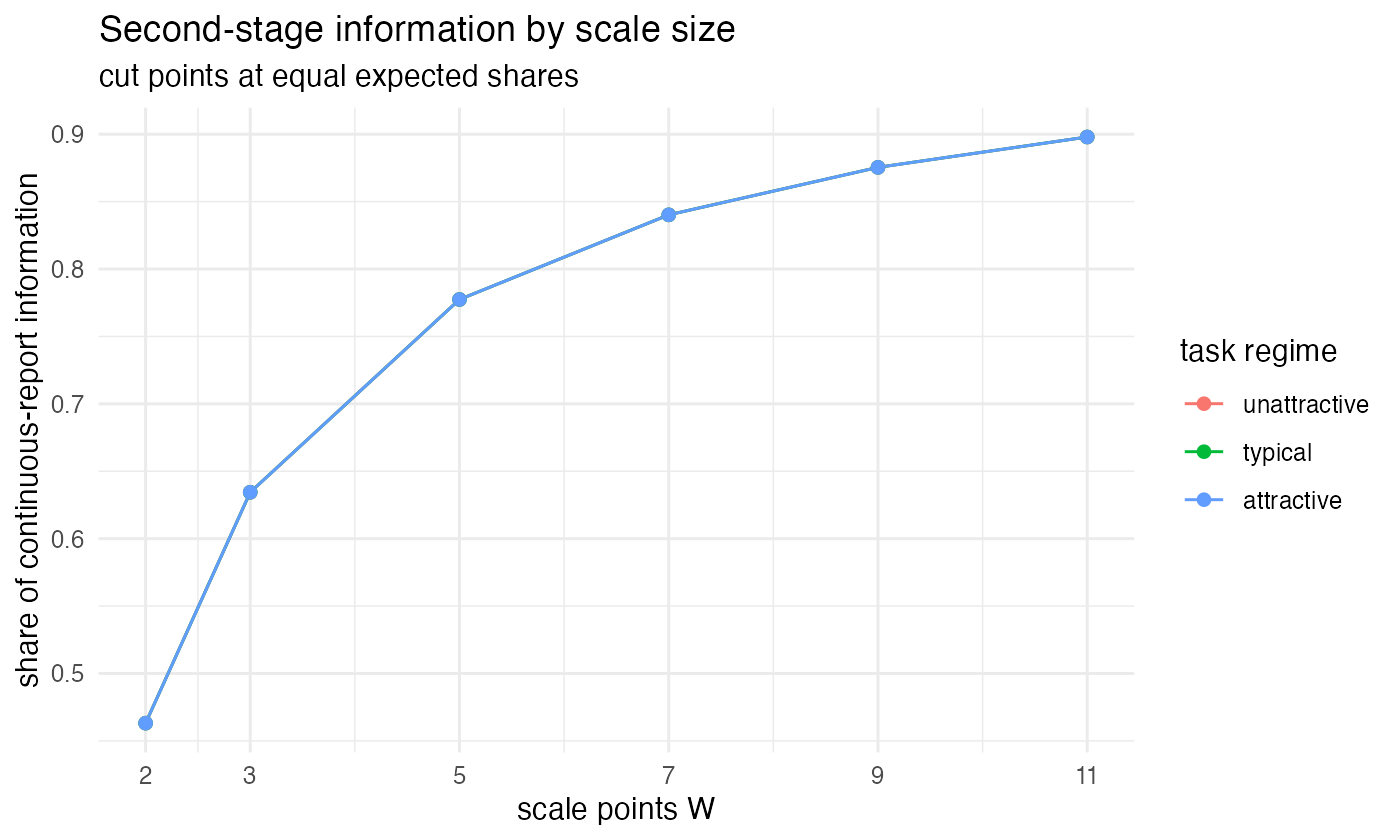
\includegraphics[width=4.67in,height=\textheight,keepaspectratio]{R/output/figs/info_by_W.png}

}

\caption{\label{fig-infoW}Share of the continuous-report information
captured by a W-point second response (cut points at equal expected
shares). The binary response is the least informative member of the
family; most of the gap closes by five points. From notebook 7.}

\end{figure}%

\textsubscript{Source:
\href{https://dyavorsky.github.io/ordinalDualresponse_paper/index.qmd.html}{Article
Notebook}}

\subsection{Economic Stakes: A Pricing
Counterfactual}\label{sec-sim-counterfactual}

Finally, \href{notebooks/08-pricing-counterfactual.qmd}{notebook 8}
pushes each estimator through the decision it exists to inform. A
synthetic market of five brands with a quality attribute, wide price
variation, and heterogeneous preferences calibrated to own-price
elasticities of about -1.9 generates \(W = 5\) dual-response data
(\(N = 500\), \(T = 12\)); each estimator's demand system then sets Nash
equilibrium prices by damped best responses, verified from multiple
starts. Demand is defined identically for all systems as top-2-box
purchase, so the well-placed binary estimator is answering exactly the
right question, and posterior-predictive demand uses full parameter
draws rather than posterior means, which would flatten heterogeneity.

\begin{longtable}[]{@{}
  >{\raggedright\arraybackslash}p{(\linewidth - 8\tabcolsep) * \real{0.1111}}
  >{\raggedleft\arraybackslash}p{(\linewidth - 8\tabcolsep) * \real{0.2685}}
  >{\raggedleft\arraybackslash}p{(\linewidth - 8\tabcolsep) * \real{0.2593}}
  >{\raggedleft\arraybackslash}p{(\linewidth - 8\tabcolsep) * \real{0.2037}}
  >{\raggedleft\arraybackslash}p{(\linewidth - 8\tabcolsep) * \real{0.1574}}@{}}

\caption{\label{tbl-counterfactual}Nash-pricing distortions by
estimator: mean and max absolute equilibrium-price error versus the true
equilibrium; error in the system's own profit forecast at its
equilibrium; and realized profit forgone relative to pricing at the true
equilibrium. Full study in notebook 8.}

\tabularnewline

\toprule\noalign{}
\begin{minipage}[b]{\linewidth}\raggedright
system
\end{minipage} & \begin{minipage}[b]{\linewidth}\raggedleft
mean \textbar price err\textbar{} \%
\end{minipage} & \begin{minipage}[b]{\linewidth}\raggedleft
max \textbar price err\textbar{} \%
\end{minipage} & \begin{minipage}[b]{\linewidth}\raggedleft
profit forecast err \%
\end{minipage} & \begin{minipage}[b]{\linewidth}\raggedleft
profit forgone \%
\end{minipage} \\
\midrule\noalign{}
\endhead
\bottomrule\noalign{}
\endlastfoot
ordinal & 1.11 & 2.13 & -2.98 & 0.37 \\
bin\_t2b & 1.10 & 2.38 & -2.47 & -0.31 \\
bin\_top & 2.57 & 5.73 & -59.29 & -0.84 \\
heur\_juster & 4.84 & 8.52 & 105.82 & 2.18 \\
heur\_t2b & 4.84 & 8.52 & 52.94 & 2.18 \\

\end{longtable}

\textsubscript{Source:
\href{https://dyavorsky.github.io/ordinalDualresponse_paper/index.qmd.html}{Article
Notebook}}

Three lessons (Table~\ref{tbl-counterfactual}). First, the full ordinal
model prices the market almost exactly. Second, the \emph{well-placed}
binary dual response also prices well, consistent with the efficiency
analysis, but the analyst does not get to choose the placement after the
fact: dichotomizing at the top box misprices by up to 5.7\% and
misstates its own profit forecast by 59\%, because a top-box model can
only answer a top-box question. Third, the constant-probability
heuristic is the expensive shortcut. Its purchase incidence cannot
respond to price, so it underprices systematically, its equilibrium
being the inside-good-only equilibrium because the calibration constant
cancels from every best response, and it overstates forecast profits by
106\%. The heuristic's failure is structural, not statistical: the
constant is the problem, so no choice of constant and no amount of data
repairs it.

\section{Empirical Application}\label{sec-analysis}

We illustrate the model with data from a commercial choice-based
conjoint study conducted in partnership with a consumer insights
consultancy, in which each choice task was followed by an ordinal
purchase-likelihood question.

\subsection{Data}\label{sec-data}

\subsection{Model Specifications and
Estimation}\label{sec-empirical-spec}

We estimate four specifications on the same data: our model
(Section~\ref{sec-model}) in aggregate and hierarchical form; the binary
dual-response benchmark applied to the dichotomized scale (top-two-box);
and the constant-probability heuristic. Hierarchical specifications use
the sampler of Section~\ref{sec-estimation}.

\textbf{Pre-specified test battery.} Before any model comparison, we
commit to the three specification tests of Section~\ref{sec-spectests}
on the aggregate fit: the unit-slope test (\(\lambda = 1\)), the
conditioning test (\(\delta = 0\)), and the DR-2Max test
(\(\delta = 1\)) --- whose operating characteristics are established in
Section~\ref{sec-sim-spectests} --- together with the A-versus-B link
comparison by holdout likelihood and WAIC. We also pre-commit to
re-running the pricing counterfactual of
Section~\ref{sec-sim-counterfactual} on the empirical posteriors,
replacing the synthetic market with the study's own category structure.

\subsection{Results}\label{sec-empirical-results}

\subsection{Scale-Usage Heterogeneity}\label{sec-empirical-hetcut}

\section{Discussion}\label{sec-discussion}

\subsection{What the Behavioral Model
Changes}\label{what-the-behavioral-model-changes}

The premise that the consumer observes everything about the inside goods
but not the outside-good shock does more than motivate a likelihood; it
reorganizes how the dual-response literature's models relate to one
another. In the binary literature, the choice between DR-2Max and
DR-AnyMax was framed as a question about the second question's wording
--- whether the respondent evaluates her selected option or the whole
set (Diener et al. 2006) --- and the shared-error Unified Model of Hung,
Liu, et al. (2025) was motivated by the internal consistency of a single
utility draw. Our framework arrives at the inclusive-value form from the
primitive assumption about information: because the maximum of Gumbel
utilities is independent of which good attains it, \emph{any} coherent
report about the best option's standing against the outside good must
depend on the task only through its inclusive value. The empirical
success of the AnyMax/Unified form over DR-2Max, documented in both
Diener et al. (2006) and Hung, Liu, et al. (2025), is what this
framework predicts. Where our account differs from Brazell et al. (2006)
is in what the second response \emph{is}: not a second choice from an
augmented set, but a report about an unresolved comparison --- which is
what licenses asking for it on an ordinal scale in the first place.

The choice of link is, likewise, a substantive behavioral question
dressed as a specification detail. It is also a question with a definite
scope. For a binary follow-up both accounts are coherent and they
disagree: resolving the outside-good draw first recovers the standard
logit second stage, while our model implies a complementary log-log one
even for yes/no data. Because the two diverge mainly in the tails,
telling them apart requires either large samples or designs with wide
variation in task attractiveness; Section~\ref{sec-analysis} provides
evidence from one commercial dataset, and we regard the question as open
and worth testing on the many existing binary dual-response datasets,
where our model's binary case can be estimated with a one-line change to
current code. For an ordinal follow-up the question does not arise in
the same form, since a respondent who has resolved the outside good
holds no graded likelihood to report.

\subsection{Implications for Practice}\label{implications-for-practice}

Four points bear directly on applied work. First, if an ordinal dual
response has been fielded, dichotomizing it is costly and arbitrary: the
analyst's choice of cut is made before seeing the data, the penalty
ranges from a few percent of sample at a lucky cut to a third of it at
an unlucky one (Section~\ref{sec-sim-benchmarks}), the damage
concentrates at the individual level where hierarchical estimation
lives, and a dichotomized model can answer questions only at its own
threshold --- the pricing counterfactual's top-box analyst misstates the
profit forecast by more than half for exactly that reason. Second,
constant-probability weighting has a \emph{structural} flaw, not a
statistical one: beyond the set-dependence of scale-point meaning
(Equation~\ref{eq-modelA} and Table~\ref{tbl-toy}), a fixed purchase
incidence cancels out of every pricing first-order condition, so the
heuristic's price recommendations ignore the no-buy margin entirely ---
no amount of data fixes this. Third, the information results in
Section~\ref{sec-information} and Section~\ref{sec-sim-design} give
concrete design guidance: five scale points capture most of the
binary-to-continuous information gap (about 78\%, versus 46\% for
binary), gains beyond seven points are small, and \emph{where} the
labels place the cut points matters as much as how many there are.
Fourth, studies that intend to test the behavioral model (the link, the
unit slope) should engineer variation in task attractiveness; designs
without it cannot discriminate the links even in principle
(Section~\ref{sec-identification}), a fact our squashed-design
experiment confirms empirically.

\subsection{Relation to the Outside-Good
Literature}\label{relation-to-the-outside-good-literature}

Our model holds the outside good's \emph{mean} utility fixed at zero and
locates all action in the consumer's uncertainty about its realization.
Two adjacent strands suggest natural extensions. Hung, Liu, et al.
(2025) show that a budget constraint applied to the second response ---
but not the forced choice --- improves fit and materially changes
equilibrium price predictions; the same asymmetric treatment is
available here, censoring the ordinal report for options priced above a
respondent-level budget, and the ordinal response should sharpen the
identification of that budget since near-threshold options will earn
lukewarm rather than merely negative reports. Hung, Kurz, et al. (2025)
document that the no-choice option's utility can drift over the course
of a survey as respondents learn about the category; in our notation
this is drift in the cut points (or in the outside-good location), and
the task-order diagnostics of Section~\ref{sec-data} carry over
directly. More broadly, the opt-out literature's warning that a single
constant rarely captures heterogeneous non-purchase behavior (Campbell
and Erdem 2019; Haaijer et al. 2001) applies to the dual response as
well; the heterogeneous-cut-point extension of Section~\ref{sec-hetcut}
is one response, and richer structures (e.g., serial non-purchasers as a
latent class) are compatible with the framework.

\subsection{Limitations}\label{limitations}

Five limitations qualify the results. First, the Gumbel error assumption
is load-bearing: the factorization of the joint likelihood and the
inclusive-value form of the second response both rest on max-stability.
Appendix D shows how far this can be pushed. Any generalized extreme
value structure, nested logit included, preserves both properties once
the inclusive value is redefined as the GEV generator, so correlation
among the displayed alternatives costs the framework nothing. Error
families outside that class do break the closed form: under a probit or
a mixed logit with a correlated kernel the max utility has no
closed-form distribution, and the second response would require
simulation over it. Our robustness experiments soften the concern in one
direction: with variance-matched normal errors, preference and demand
estimates are essentially unimpaired, the misspecification being
absorbed by the cut-point locations --- so structural interpretation of
the cut points deserves more caution than the demand quantities built
from them. Second, we treat tasks as independent draws, abstracting from
learning, fatigue, and reference formation across the sequence (Hung,
Kurz, et al. 2025); the task-order diagnostic of
Section~\ref{sec-sim-robust} detects such drift reliably when present.
Third, the common-cut-point model assumes a shared reading of the scale
labels; the extension of Section~\ref{sec-hetcut} relaxes this, but
individual-level identification is thin at commercial task counts, and
our simulations find that ignoring moderate scale-usage heterogeneity
costs little --- the extension earns its keep as insurance and as a
diagnostic, not as a default. Fourth, like all stated-preference
methods, the model calibrates stated rather than revealed purchase
behavior; the ordinal report inherits whatever hypothetical bias attends
purchase-intent questions generally (Morrison 1979), and linking the
estimated cut points to realized purchase rates --- the ordinal analogue
of the calibration literature on binary intentions --- is a natural next
step. Fifth, the likelihood presumes the two questions are asked
together, as in the standard dual-response task. Designs that separate
them, such as the separated dual response of Schlereth and Skiera
(2017), break the coupling between the two responses and would require
the stages to be modeled as separate draws. A separate methodological
caution, documented in Appendix C, is that harmonic-mean
marginal-likelihood estimates are optimistic; we therefore anchor model
comparisons in holdout likelihood and WAIC alongside the conventional
estimator.

\section{Conclusion}\label{sec-conclusion}

Dual-response conjoint separates a question consumers answer readily,
which of these do you like best, from one they cannot answer with
certainty, would you actually buy it. This paper takes that uncertainty
as the modeling primitive. A consumer who observes everything about the
displayed alternatives but not her valuation of the outside good holds a
purchase probability rather than a decision, so the natural follow-up
question is ordinal and the natural model joins a multinomial logit for
the forced choice to a cumulative-link ordinal model on the task's
inclusive value. The link function is not a modeling choice. It follows
from whether the respondent reports the probability she still holds, as
our model has her do, or resolves her uncertainty and grades the
comparison that results, and the two are distinguishable on data that
vary the attractiveness of the displayed alternatives.

Three results follow. At two scale points the logistic link is the
incumbent binary dual-response model, so the ordinal form is an
extension of that literature rather than a departure from it, while our
model's binary case is a complementary log-log response, which implies
that the familiar yes/no follow-up is mildly misspecified and can be
checked on data already collected. A finer scale never subtracts
information, and five points capture most of the gap between a binary
answer and a continuous one. The two ways an ordinal answer is otherwise
reduced to something the binary model accepts, collapsing the scale at
an arbitrary point and assigning each point a fixed purchase
probability, are respectively wasteful and internally inconsistent, the
second because the meaning of a scale label depends on what was on the
screen. Simulation evidence confirms that the aggregate and hierarchical
Bayesian estimators recover the model's parameters, including the cut
points that give the scale labels quantitative meaning, and that the
conclusions survive correlated alternatives, non-Gumbel errors, and
drift in the outside good across a respondent's task sequence.

The broader point is that a response format and the model that reads it
belong together. A finer scale is worth fielding only if something can
use the extra categories, and a model is worth deriving only if the
question it reads is one respondents can answer. Supplying the
likelihood makes the ordinal follow-up a measurement instrument rather
than a longer question, and it opens work on calibrating estimated cut
points against realized purchase behavior, on using the ordinal response
to identify budget constraints, and on the design of the scale itself.

\section*{Appendix A: Proofs}\label{sec-appendix-proofs}
\addcontentsline{toc}{section}{Appendix A: Proofs}

\subsection*{\texorpdfstring{A.1 Proof of
Lemma~\ref{lem-gumbel}}{A.1 Proof of Lemma~}}\label{a.1-proof-of-lem-gumbel}
\addcontentsline{toc}{subsection}{A.1 Proof of Lemma~\ref{lem-gumbel}}

Let \(u_j = V_j + \eta_j\) with \(\eta_j \iid \text{Gumbel}(0,1)\) for
\(j \in \mathcal{J}^+\), so \(u_j\) has CDF
\(F_j(t) = \exp\left( -e^{-(t - V_j)} \right)\) and density
\(f_j(t) = e^{-(t-V_j)} \exp\left( -e^{-(t-V_j)} \right)\). For any
\(j\) and any \(u\), \[
\Pr \left( j^* = j, \; u^* \le u \right)
= \int_{-\infty}^{u} f_j(t) \prod_{k \ne j} F_k(t) \, dt
= \int_{-\infty}^{u} e^{V_j} e^{-t} \exp \left( -e^{-t} S \right) dt,
\] using
\(\prod_{k \ne j} F_k(t) = \exp\left( -e^{-t} \left( S - e^{V_j} \right) \right)\)
with \(S = \sum_{k} e^{V_k}\), and collecting terms. Substituting
\(s = e^{-t} S\) (so \(ds = -e^{-t} S \, dt\)) gives \[
\Pr \left( j^* = j, \; u^* \le u \right)
= \frac{e^{V_j}}{S} \int_{e^{-u} S}^{\infty} e^{-s} \, ds
= \underbrace{\frac{e^{V_j}}{S}}_{\Pr\left(j^*=j\right)} \; \times \; \underbrace{\exp \left( -S e^{-u} \right)}_{F_{\text{Gumbel}\left(\overline{\mu},1\right)}(u)}.
\] Letting \(u \to \infty\) delivers the MNL choice probability; summing
over \(j\) delivers \(u^* \sim \text{Gumbel}(\overline{\mu}, 1)\) with
\(\overline{\mu} = \ln S\); and the factorization of the joint law for
every \((j, u)\) is precisely the independence of \(j^*\) and \(u^*\).
\(\square\)

The calculation above is short but gives little sense of why the two
quantities separate. The following change of variable makes it
transparent, and it is the same argument that generalizes to correlated
alternatives in Appendix D.

Write \(y_j = e^{V_j}\) and set \(T_j = e^{-u_j}\). The map is
decreasing, so it exchanges maxima for minima: the best good is the one
with the smallest \(T_j\), and \(u^* = -\ln \min_j T_j\). Under the
Gumbel assumption, \[
\Pr \left( T_j > t \right) = \Pr \left( u_j < -\ln t \right) = e^{-y_j t},
\] so each good becomes an independent waiting time that arrives at the
constant rate \(y_j\), and the consumer's chosen good is whichever
arrives first.

For independent waiting times of this kind, the identity of the first
arrival and the time of that arrival are independent, and the reason is
that the rates do not change as time passes. At any instant, given that
nothing has yet arrived, the chance that the next arrival is good \(j\)
is \(y_j / S\), the same at the start as at any later point. Which good
arrives first is therefore settled entirely by the rates relative to one
another, while how long the wait lasts is settled entirely by their sum
\(S\). Waiting longer says nothing about who will win. Transforming
back, the shares \(y_j / S\) are the multinomial logit probabilities and
the total \(S\) fixes the location of \(u^*\), which is the content of
Lemma~\ref{lem-gumbel}. This is the division of labor between the two
responses. The rates relative to one another are the utility differences
that the forced choice reveals, and their sum is the inclusive value
that the ordinal report reads, so the two responses read separate
features of the same draw.

The same statement in utility terms is that the relative odds of being
the maximizer are the same at every level of the maximum, because Gumbel
upper tails decay exponentially and are therefore shift-invariant:
\(\Pr(u_1 > m) / \Pr(u_2 > m) = e^{V_1 - V_2}\) for every \(m\).

This is a property of the extreme-value family and not of random utility
models in general. Under normal errors with \(V_1 > V_2\), the ratio of
upper tails diverges as \(m\) grows, so a high realized maximum is
disproportionately likely to have come from the better alternative. The
level of the maximum then carries information about which alternative
attained it, the joint law of \(\left( j^*, u^* \right)\) does not
factor, and the counterpart of Equation~\ref{eq-joint} is unavailable.
What Appendix D shows is that the factorization survives correlation
among the inside goods, because the waiting times may be dependent and
still arrive at rates whose ratios are constant over time; what fails
outside the extreme-value family is the constancy of those ratios.

\subsection*{\texorpdfstring{A.2 Derivation of the information increment
(Equation~\ref{eq-fisher})}{A.2 Derivation of the information increment (Equation~)}}\label{a.2-derivation-of-the-information-increment-eq-fisher}
\addcontentsline{toc}{subsection}{A.2 Derivation of the information
increment (Equation~\ref{eq-fisher})}

The second response contributes the multinomial log-likelihood
\(\ell = \sum_w \mathbb{1}\lbrace y = w \rbrace \ln \pi_w\) with
\(\pi_w = G(c_w - \overline{\mu}) - G(c_{w-1} - \overline{\mu})\). Since
\(\partial \overline{\mu} / \partial \bfbeta = \sum_j \Pr(j^* = j) \, \x_j = \overline{\x}\),
the score with respect to \(\bfbeta\) in category \(w\) is
\(- \left[ g_w - g_{w-1} \right] / \pi_w \cdot \overline{\x}\), writing
\(g_w = g \left( c_w - \overline{\mu} \right)\) and \(g = G'\) (with
\(g_0 = g_W = 0\)). The information is the expected outer product of the
score: \[
\mathcal{I}^{(2)} = \sum_{w=1}^{W} \pi_w \left( \frac{g_w - g_{w-1}}{\pi_w} \right)^2 \overline{\x} \, \overline{\x}'
= \left[ \sum_{w=1}^{W} \frac{ \left( g_w - g_{w-1} \right)^2 }{ \pi_w } \right] \overline{\x} \, \overline{\x}'
= \omega \left( \overline{\mu}; \mathbf{c} \right) \overline{\x} \, \overline{\x}'. \qquad \square
\] The joint information over \(\left( \bfbeta, \mathbf{c} \right)\),
including the cut-point blocks used by the estimation code, follows from
the same score with
\(\partial \pi_w / \partial c_m = g_w \mathbb{1}\lbrace m = w \rbrace - g_{w-1} \mathbb{1}\lbrace m = w-1 \rbrace\).

\subsection*{\texorpdfstring{A.3 Monotonicity of \(\omega\) under
refinement}{A.3 Monotonicity of \textbackslash omega under refinement}}\label{a.3-monotonicity-of-omega-under-refinement}
\addcontentsline{toc}{subsection}{A.3 Monotonicity of \(\omega\) under
refinement}

Let \(\mathcal{C}'\) be a coarsening of the partition \(\mathcal{C}\)
obtained by merging adjacent categories \(w\) and \(w+1\). The merged
cell contributes
\(\left( g_{w+1} - g_{w-1} \right)^2 / \left( \pi_w + \pi_{w+1} \right)\)
to \(\omega'\), while the two original cells contribute
\(\left( g_w - g_{w-1} \right)^2 / \pi_w + \left( g_{w+1} - g_w \right)^2 / \pi_{w+1}\)
to \(\omega\). Writing \(a = g_w - g_{w-1}\), \(b = g_{w+1} - g_w\),
\(u = \pi_w\), \(v = \pi_{w+1}\), the Cauchy--Schwarz inequality in
Engel form gives \[
\frac{(a + b)^2}{u + v} \;\le\; \frac{a^2}{u} + \frac{b^2}{v},
\] so each merge weakly decreases \(\omega\), and any coarsening ---
being a finite sequence of adjacent merges --- does the same. The binary
response is the coarsest member of the family and hence the least
informative; conversely, as the mesh of the partition goes to zero the
interval score converges to the exact-observation score and
\(\omega \to \int \left( g' \right)^2 / g \, dz\), the Fisher
information of the latent's location (equal to \(1\) for the standard
Gumbel and \(1/3\) for the standard logistic). \(\square\)

\section*{Appendix B: Estimation Details}\label{sec-appendix-estimation}
\addcontentsline{toc}{section}{Appendix B: Estimation Details}

\textbf{Aggregate model.} The likelihood is maximized over the working
parameters
\(\left( \bfbeta, c_1, \ln(c_2 - c_1), \ldots, \ln(c_{W-1} - c_{W-2}) \right)\),
which enforce cut-point monotonicity without constraints; standard
errors for the cut points follow by the delta method. Interval
probabilities are computed with tail-stable expressions
(\(\Lambda(h)\Lambda(-l)(1 - e^{l-h})\) for the logistic link and
\(e^{-e^{-h}}\left(1 - e^{-(e^{-l} - e^{-h})}\right)\) for the Gumbel
link) so that extreme cut points do not lose precision to cancellation.

\textbf{Hierarchical model.} The sampler is a random-walk
Metropolis-within-Gibbs in the style of Rossi et al. (2005) with three
blocks per iteration: (1) all respondents' \(\bfbeta_i\) (and, in the
heterogeneous-cut-point extension, \(\bftheta_i\)) are updated
simultaneously by independent normal random-walk proposals with
covariance \(s_i^2 \Sigma\); (2) the common cut-point block is updated
by a random-walk proposal on the unconstrained scale; (3) the population
moments \(\left( \betabar, \Sigma \right)\) are drawn from their
conjugate normal and inverse-Wishart conditionals. Priors:
\(\betabar \sim \mathcal{N}\left( \mathbf{0}, 100 I \right)\),
\(\Sigma \sim \text{IW}\left( \dim + 3, (\dim + 3) I \right)\), and
\(\mathcal{N}(0, 100 I)\) on the transformed cut points. Step sizes are
initialized at \(2.93/\sqrt{\dim}\) and adapted only during burn-in
toward acceptance rates of \(0.23\) (individual blocks) and \(0.30\)
(cut-point block). Unless noted, we run 30,000 iterations, discard
10,000, and keep every 10th draw.

The sampler was validated four ways (replication code accompanies the
paper): parameter recovery on synthetic panels for both links;
repeated-sampling coverage of 50\% and 90\% posterior intervals at
nominal rates; agreement of the forced-choice-only special case with an
independent hierarchical-MNL implementation (posterior means matching to
less than 0.01 on all hyperparameters on common data); and convergence
of the posterior toward the aggregate MLE when the data are generated
without heterogeneity.

\section*{Appendix C: Marginal-Likelihood
Estimation}\label{sec-appendix-lmd}
\addcontentsline{toc}{section}{Appendix C: Marginal-Likelihood
Estimation}

Model comparisons in the paper report the log marginal density (LMD).
For hierarchical models we follow the standard practice in this
literature (Hung, Liu, et al. 2025) and use the harmonic-mean estimator
of Newton and Raftery (1994), complemented by two quantities that do not
rely on it: the WAIC computed from pointwise per-respondent likelihoods
(Watanabe 2010; Vehtari et al. 2017) and the log posterior-predictive
density of held-out tasks. The reason for the complements is that the
harmonic-mean estimator is optimistic. In the aggregate model --- where
the parameter space is small enough for exact methods --- we can
quantify this directly: bridge sampling (Meng and Wong 1996; Gronau et
al. 2020) and a Laplace approximation agree with each other to well
under one log point, while the Newton--Raftery estimate exceeds them by
dozens of log points, and trimming the smallest-likelihood draws widens
rather than closes the gap:

\begin{longtable}[]{@{}lrr@{}}

\caption{\label{tbl-lmd-check}Aggregate-model log marginal density by
estimator (simulated data, n = 3,600 tasks; from notebook 03).}

\tabularnewline

\toprule\noalign{}
estimator & log marginal density & vs.~bridge \\
\midrule\noalign{}
\endhead
\bottomrule\noalign{}
\endlastfoot
bridge & -9844.14 & 0.00 \\
laplace & -9844.15 & -0.01 \\
NR & -9801.78 & 42.36 \\
NR trim 5\% & -9799.63 & 44.51 \\
NR trim 20\% & -9798.42 & 45.73 \\

\end{longtable}

\textsubscript{Source:
\href{https://dyavorsky.github.io/ordinalDualresponse_paper/index.qmd.html}{Article
Notebook}}

Because the bias is similar for models of similar dimension,
Newton--Raftery \emph{rankings} between the ordinal and binary
dual-response models are typically preserved --- but we treat the WAIC
and holdout comparisons as primary whenever the two disagree.

\section*{Appendix D: Correlated Alternatives}\label{sec-appendix-gev}
\addcontentsline{toc}{section}{Appendix D: Correlated Alternatives}

Lemma~\ref{lem-gumbel} is stated for independent Gumbel errors, and the
whole of Section~\ref{sec-model} rests on it. This appendix shows that
both of its properties hold for the entire generalized extreme value
(GEV) family of McFadden (1981), so that correlation among the inside
goods costs the framework nothing beyond a redefinition of the inclusive
value.

Let the inside-good components have the GEV joint distribution
\begin{equation}\protect\phantomsection\label{eq-gevcdf}{
\Pr \left( \eta_1 \le e_1, \ldots, \eta_J \le e_J \right)
= \exp \left( - G \left( e^{-e_1}, \ldots, e^{-e_J} \right) \right),
}\end{equation} where the generator
\(G : \mathbb{R}^J_{+} \to \mathbb{R}_{+}\) is homogeneous of degree
one, tends to infinity in each argument, and has mixed partial
derivatives that alternate in sign. Independent Gumbel errors are the
special case \(G(y) = \sum_j y_j\). Write \(y_j = \exp(V_j)\),
\(G_j = \partial G / \partial y_j\), and
\begin{equation}\protect\phantomsection\label{eq-gevmu}{
S^{G} \coloneqq G \left( y_1, \ldots, y_J \right),
\qquad
\overline{\mu} \coloneqq \ln S^{G}.
}\end{equation}

\begin{lemma}[]\protect\hypertarget{lem-gev}{}\label{lem-gev}

Under Equation~\ref{eq-gevcdf}, with \(u_j = V_j + \eta_j\) and
\(u^* = \max_{j} u_j\):

\begin{enumerate}
\def\labelenumi{(\roman{enumi})}
\item
  \(u^* \sim \text{Gumbel} \left( \overline{\mu}, 1 \right)\) with
  \(\overline{\mu} = \ln S^{G}\);
\item
  \(j^*\) and \(u^*\) are statistically independent, with
  \(\Pr(j^* = j) = y_j G_j(y) / S^{G}\).
\end{enumerate}

\end{lemma}

\begin{proof}
The joint CDF of the utilities is \[
H \left( m_1, \ldots, m_J \right)
= \exp \left( - G \left( y_1 e^{-m_1}, \ldots, y_J e^{-m_J} \right) \right).
\] For (i), set every \(m_j = m\) and use homogeneity of degree one:
\(G(y e^{-m}) = e^{-m} G(y)\), so
\(H(m, \ldots, m) = \exp \left( - e^{-m} S^{G} \right)\), which is the
\(\text{Gumbel}\left(\ln S^{G}, 1\right)\) CDF.

For (ii), write \(t_k = y_k e^{-m_k}\) and differentiate: \[
\frac{\partial H}{\partial m_j}
= \exp \left( -G(t) \right) \, G_j(t) \, y_j e^{-m_j}.
\] Because \(G\) is homogeneous of degree one, \(G_j\) is homogeneous of
degree zero, so evaluating at \(m_k = s\) for every \(k\) gives
\(G_j(t) = G_j(y)\) and \(G(t) = e^{-s} S^{G}\). Hence \[
\left. \frac{\partial H}{\partial m_j} \right|_{m_k = s \ \forall k}
= \exp \left( - e^{-s} S^{G} \right) G_j(y) \, y_j e^{-s}
= \frac{y_j G_j(y)}{S^{G}} \cdot \frac{d}{ds} \exp \left( - e^{-s} S^{G} \right),
\] and integrating from \(-\infty\) to \(u\), \[
\Pr \left( j^* = j, \ u^* \le u \right)
= \underbrace{\frac{y_j G_j(y)}{S^{G}}}_{\Pr \left( j^* = j \right)}
\; \times \;
\underbrace{\exp \left( - e^{-u} S^{G} \right)}_{\Pr \left( u^* \le u \right)}
\] for every \(j\) and every \(u\), which is the claimed independence.
Letting \(u \to \infty\) recovers the GEV choice probability.
\(\square\)
\end{proof}

Everything in Section~\ref{sec-model} follows with \(S_{it}\) replaced
by \(S^{G}_{it}\). The first response becomes the GEV choice probability
rather than the multinomial logit; the second response is unchanged in
form, since Equation~\ref{eq-modelA}, Equation~\ref{eq-modelB}, and the
cumulative-link representation Equation~\ref{eq-cumlink} depend on the
choice set only through \(\overline{\mu}_{it}\); and the factorization
Equation~\ref{eq-joint} holds for the same reason as before. The
location invariance behind Proposition~\ref{prp-ident} also survives:
shifting every \(V_{itj}\) by \(\delta\) multiplies \(S^{G}_{it}\) by
\(e^{\delta}\) and so shifts \(\overline{\mu}_{it}\) by exactly
\(\delta\), which the cut points absorb. The rank condition must then be
read against the design as it enters \(G\) rather than a simple sum, and
the nesting result of Section~\ref{sec-nesting} becomes
\(\Pr(\text{buy}) = S^{G}_{it} / \left( e^{\gamma} + S^{G}_{it} \right)\).

The leading application is nested logit,
\(G(y) = \sum_{n} \left( \sum_{j \in n} y_j^{1/\lambda_n} \right)^{\lambda_n}\),
in which alternatives within a nest are correlated whenever
\(\lambda_n < 1\). We confirm Lemma~\ref{lem-gev} numerically for a
five-alternative, two-nest design with \(\lambda = (0.5, 0.8)\) using
the positive-stable mixture representation of the nested logit
(\texttt{R/homogeneous/gev\_check.R}). Across two million draws the
simulated distribution of \(u^*\) matches
\(\text{Gumbel}(\ln S^{G}, 1)\) (location \(1.845\) against \(1.846\)
analytically; Kolmogorov-Smirnov \(p = 0.17\)), the simulated choice
shares match \(y_j G_j / S^{G}\) to four decimal places, and the
conditional distribution of \(u^*\) given \(j^*\) is indistinguishable
from its unconditional counterpart at every quartile (chi-square test of
independence, \(p = 0.70\)).

Two limits of the result are worth stating. It covers correlation among
the \emph{inside} goods only: the outside-good shock \(\eta_{it0}\) is
assumed independent of them throughout, and The logistic link uses that
independence to obtain
\(d_{it} \sim \text{Logistic}(\overline{\mu}_{it}, 1)\). And it does not
extend to error structures outside the GEV class, such as multinomial
probit or a mixed logit with correlated kernel errors, for which \(u^*\)
has no closed-form distribution and the factorization that makes
Equation~\ref{eq-joint} tractable is unavailable.

\section*{Appendix E: Implementation in
Apollo}\label{sec-appendix-apollo}
\addcontentsline{toc}{section}{Appendix E: Implementation in Apollo}

\textsubscript{Source:
\href{https://dyavorsky.github.io/ordinalDualresponse_paper/index.qmd.html}{Article
Notebook}}

The replication archive implements the model twice: once directly, in
the routines described in Appendix B, and once in Apollo (Hess and Palma
2019), the freeware choice-modelling package for R. The second
implementation serves two purposes. It cross-validates our code against
an independently developed and widely used toolkit, and it shows how the
model fits into an estimation framework readers are likely to already
have installed.

\textbf{The model as a two-component structure.} Apollo builds a
likelihood by multiplying components. Our joint likelihood
Equation~\ref{eq-joint} is exactly of that form, so the forced choice is
an \texttt{apollo\_mnl} component and the ordinal follow-up is a second
component over the same tasks. This is the architecture of the hybrid
choice models for which the package is often used, in which a
multinomial logit for the choice is combined with ordered-response
components for attitudinal indicators (Daly et al. 2012). The
resemblance is worth being precise about, because the difference is the
content of Section~\ref{sec-model}. In a hybrid choice model the ordinal
component is driven by a latent attitude that is exogenous to the
choice, and it is connected to the choice utilities through freely
estimated loading parameters. Here the ordinal component is driven by
the inclusive value of the same choice set, and its loading is fixed at
one rather than estimated. Our model is the restricted case, and
Lemma~\ref{lem-gumbel} is what licenses the restriction.

\textbf{The logistic specification is native; ours is not.} With the
second stage a cumulative logit in \(\overline{\mu}_{it}\), The logistic
specification is assembled from stock parts: \texttt{apollo\_mnl} for
the choice, \texttt{apollo\_ol} for the follow-up with the task's
inclusive value passed as its single explanatory variable and the cut
points as its thresholds, and \texttt{apollo\_combineModels} to join
them. Our model has no stock part. Apollo supplies ordered components
for the logistic and normal links and no others, so the
complementary-log-log form Equation~\ref{eq-modelA} must be written out
and passed through \texttt{apollo\_ownModel}, the hook for user-defined
likelihoods. This is a small piece of code, and once supplied it
inherits the rest of the package. The asymmetry is worth noting for its
own sake: the standard toolkit anticipates the behavior in which the
respondent resolves her uncertainty before answering, and not the
behavior in which she reports the probability she still holds.

\textbf{Agreement.} Table~\ref{tbl-apollo} reports the largest
discrepancy between the two implementations over 5 independent datasets
of 2,000 tasks in each of two configurations, with both implementations
started from the same values.

\begin{longtable}[]{@{}
  >{\raggedright\arraybackslash}p{(\linewidth - 10\tabcolsep) * \real{0.2747}}
  >{\raggedright\arraybackslash}p{(\linewidth - 10\tabcolsep) * \real{0.1978}}
  >{\raggedright\arraybackslash}p{(\linewidth - 10\tabcolsep) * \real{0.0659}}
  >{\raggedright\arraybackslash}p{(\linewidth - 10\tabcolsep) * \real{0.1209}}
  >{\raggedright\arraybackslash}p{(\linewidth - 10\tabcolsep) * \real{0.1758}}
  >{\raggedright\arraybackslash}p{(\linewidth - 10\tabcolsep) * \real{0.1648}}@{}}

\caption{\label{tbl-apollo}Largest absolute discrepancy between our
maximum-likelihood routine and the same model estimated in Apollo, over
five independent datasets per configuration (from
R/apollo/compare\_apollo.R).}

\tabularnewline

\toprule\noalign{}
\begin{minipage}[b]{\linewidth}\raggedright
configuration
\end{minipage} & \begin{minipage}[b]{\linewidth}\raggedright
ordinal component
\end{minipage} & \begin{minipage}[b]{\linewidth}\raggedright
beta
\end{minipage} & \begin{minipage}[b]{\linewidth}\raggedright
cut points
\end{minipage} & \begin{minipage}[b]{\linewidth}\raggedright
standard errors
\end{minipage} & \begin{minipage}[b]{\linewidth}\raggedright
log-likelihood
\end{minipage} \\
\midrule\noalign{}
\endhead
\bottomrule\noalign{}
\endlastfoot
Our model, W = 5 & apollo\_ownModel & 1e-06 & 2e-06 & 1e-07 & 9e-10 \\
Logistic, W = 2 (binary) & apollo\_ol & 5e-07 & 5e-07 & 5e-09 & 6e-11 \\

\end{longtable}

\textsubscript{Source:
\href{https://dyavorsky.github.io/ordinalDualresponse_paper/index.qmd.html}{Article
Notebook}}

Point estimates agree to 2e-06 or better, standard errors to 1e-06, and
the maximized log-likelihood to 9e-10, which is convergence tolerance
rather than disagreement. The two implementations share no code: Apollo
computes the ordinal probabilities for our model from the direct
expression
\(e^{-e^{-(c_w - \overline{\mu})}} - e^{-e^{-(c_{w-1} - \overline{\mu})}}\),
while ours uses the tail-stable rearrangement of Appendix B, and the cut
points enter Apollo's likelihood as free parameters rather than through
the monotone increment parameterization. The binary row is the incumbent
dual-response model of Diener et al. (2006) and Hung, Liu, et al.
(2025), recovered as the two-point special case of
Section~\ref{sec-nesting}.

\textbf{Why the hierarchical model is not estimated in Apollo.} Apollo
reaches Bayesian estimation by wrapping \texttt{RSGHB}, which requires
each random parameter to be assigned one of a fixed menu of marginal
distributions: normal, log-normal, censored normal, or Johnson SB. None
of them can express an ordered vector. The heterogeneous-cut-point
extension of Section~\ref{sec-hetcut} gives each respondent her own
thresholds \(\bftheta_i\), which must stay ordered for the likelihood to
be defined, and we impose that through a transformation to an
unconstrained scale inside a random-walk block. That is expressible in a
purpose-written sampler and not in the \texttt{RSGHB} menu. The
restriction is specific to the Bayesian path: \texttt{apollo\_ol}
accepts thresholds that vary across observations, so classical
mixed-threshold specifications are available. This is the reason the
hierarchical results in Section~\ref{sec-simstudy} come from the sampler
of Appendix B rather than from Apollo.

\section*{Declaration of generative AI and AI-assisted technologies in
the manuscript preparation
process}\label{declaration-of-generative-ai-and-ai-assisted-technologies-in-the-manuscript-preparation-process}
\addcontentsline{toc}{section}{Declaration of generative AI and
AI-assisted technologies in the manuscript preparation process}

During the preparation of this work the authors used Claude (Anthropic),
accessed through Claude Code, iteratively in the drafting and editing of
manuscript text and select coding tasks. After using this tool, the
authors reviewed and edited the content as needed and take full
responsibility for the content of the published article.

\section*{References}\label{references}
\addcontentsline{toc}{section}{References}

\protect\phantomsection\label{refs}
\begin{CSLReferences}{1}{1}
\bibitem[\citeproctext]{ref-Allenby_2019}
Allenby, Greg M., Nino Hardt, and Peter E. Rossi. 2019. {``Economic
Foundations of Conjoint Analysis.''} In \emph{Handbook of the Economics
of Marketing}, edited by Jean-Pierre Dubé and Peter E. Rossi, vol. 1.
North-Holland.

\bibitem[\citeproctext]{ref-Brazell_2006}
Brazell, Jeff D., Christopher G. Diener, Ekaterina Karniouchina, William
L. Moore, Válerie Séverin, and Pierre-Francois Uldry. 2006. {``The
No-Choice Option and Dual Response Choice Designs.''} \emph{Marketing
Letters} 17 (4): 255--68.
\url{https://doi.org/10.1007/s11002-006-7943-8}.

\bibitem[\citeproctext]{ref-Bucklin_1992}
Bucklin, Randolph E., and Sunil Gupta. 1992. {``Brand Choice, Purchase
Incidence, and Segmentation: An Integrated Modeling Approach.''}
\emph{Journal of Marketing Research} 29 (2): 201--15.
\url{https://doi.org/10.1177/002224379202900205}.

\bibitem[\citeproctext]{ref-Campbell_2019}
Campbell, Danny, and Seda Erdem. 2019. {``Including Opt-Out Options in
Discrete Choice Experiments: Issues to Consider.''} \emph{The Patient -
Patient-Centered Outcomes Research} 12 (1): 1--14.
\url{https://doi.org/10.1007/s40271-018-0324-6}.

\bibitem[\citeproctext]{ref-Cardell_1997}
Cardell, N. Scott. 1997. {``Variance Components Structures for the
Extreme-Value and Logistic Distributions with Application to Models of
Heterogeneity.''} \emph{Econometric Theory} 13 (2): 185--213.
\url{https://doi.org/10.1017/s0266466600005727}.

\bibitem[\citeproctext]{ref-Daly_2012}
Daly, Andrew, Stephane Hess, Bhanu Patruni, Dimitris Potoglou, and
Charlene Rohr. 2012. {``Using Ordered Attitudinal Indicators in a Latent
Variable Choice Model: A Study of the Impact of Security on Rail Travel
Behaviour.''} \emph{Transportation} 39 (2): 267--97.
\url{https://doi.org/10.1007/s11116-011-9351-z}.

\bibitem[\citeproctext]{ref-Dhar_2003}
Dhar, Ravi, and Itamar Simonson. 2003. {``The Effect of Forced Choice on
Choice.''} \emph{Journal of Marketing Research} 40 (2): 146--60.
\url{https://doi.org/10.1509/jmkr.40.2.146.19229}.

\bibitem[\citeproctext]{ref-Diener_2006}
Diener, Christopher G., Bryan K. Orme, and David Yardley. 2006. {``Dual
Response {`None'} Approaches: Theory and Practice.''} \emph{Proceedings
of the Sawtooth Software Conference} (Sequim, WA), 157--67.

\bibitem[\citeproctext]{ref-Falco_2015}
Falco, Paolo, William F. Maloney, Bob Rijkers, and Mauricio Sarrias.
2015. {``Heterogeneity in Subjective Wellbeing: An Application to
Occupational Allocation in {Africa}.''} \emph{Journal of Economic
Behavior \& Organization} 111: 137--53.
\url{https://doi.org/10.1016/j.jebo.2014.12.022}.

\bibitem[\citeproctext]{ref-Greene_2010}
Greene, William H., and David A. Hensher. 2010. {``Ordered Choices and
Heterogeneity in Attribute Processing.''} \emph{Journal of Transport
Economics and Policy} 44 (3): 331--64.

\bibitem[\citeproctext]{ref-Gronau_2020}
Gronau, Quentin F., Henrik Singmann, and Eric-Jan Wagenmakers. 2020.
{``Bridgesampling: An {R} Package for Estimating Normalizing
Constants.''} \emph{Journal of Statistical Software} 92 (10): 1--29.
\url{https://doi.org/10.18637/jss.v092.i10}.

\bibitem[\citeproctext]{ref-Gupta_1988}
Gupta, Sunil. 1988. {``Impact of Sales Promotions on When, What, and How
Much to Buy.''} \emph{Journal of Marketing Research} 25 (4): 342--55.
\url{https://doi.org/10.1177/002224378802500402}.

\bibitem[\citeproctext]{ref-Haaijer_2001}
Haaijer, Rinus, Wagner A. Kamakura, and Michel Wedel. 2001. {``The
{`No-Choice'} Alternative in Conjoint Choice Experiments.''}
\emph{International Journal of Market Research} 43 (1): 93--106.
\url{https://doi.org/10.1177/147078530104300105}.

\bibitem[\citeproctext]{ref-Hess_2019}
Hess, Stephane, and David Palma. 2019. {``Apollo: A Flexible, Powerful
and Customisable Freeware Package for Choice Model Estimation and
Application.''} \emph{Journal of Choice Modelling} 32: 100170.
\url{https://doi.org/10.1016/j.jocm.2019.100170}.

\bibitem[\citeproctext]{ref-Huber_1996}
Huber, Joel, and Klaus Zwerina. 1996. {``The Importance of Utility
Balance in Efficient Choice Designs.''} \emph{Journal of Marketing
Research} 33 (3): 307--17.
\url{https://doi.org/10.1177/002224379603300305}.

\bibitem[\citeproctext]{ref-Hung_2025_nochoice}
Hung, Cheng-Yu, Peter Kurz, Roger A. Bailey, Joel Huber, and Greg M.
Allenby. 2025. {``Re-Examining the No-Choice Option in Conjoint
Analysis.''} \emph{Journal of Choice Modelling} 57: 100578.
\url{https://doi.org/10.1016/j.jocm.2025.100578}.

\bibitem[\citeproctext]{ref-Hung_2025_dual}
Hung, Cheng-Yu, YiChun Miriam Liu, Jeff D. Brazell, and Greg M. Allenby.
2025. {``Dual Response in Conjoint Analysis.''} \emph{Marketing Letters}
36 (4): 857--73. \url{https://doi.org/10.1007/s11002-025-09787-1}.

\bibitem[\citeproctext]{ref-Juster_1966}
Juster, F. Thomas. 1966. {``Consumer Buying Intentions and Purchase
Probability: An Experiment in Survey Design.''} \emph{Journal of the
American Statistical Association} 61 (315): 658--96.
\url{https://doi.org/10.1080/01621459.1966.10480897}.

\bibitem[\citeproctext]{ref-Manski_1990}
Manski, Charles F. 1990. {``The Use of Intentions Data to Predict
Behavior: A Best-Case Analysis.''} \emph{Journal of the American
Statistical Association} 85 (412): 934--40.
\url{https://doi.org/10.1080/01621459.1990.10474964}.

\bibitem[\citeproctext]{ref-Manski_2004}
Manski, Charles F. 2004. {``Measuring Expectations.''}
\emph{Econometrica} 72 (5): 1329--76.
\url{https://doi.org/10.1111/j.1468-0262.2004.00537.x}.

\bibitem[\citeproctext]{ref-Marshall_2002}
Marshall, Pablo, and Eric T. Bradlow. 2002. {``A Unified Approach to
Conjoint Analysis Models.''} \emph{Journal of the American Statistical
Association} 97 (459): 674--82.
\url{https://doi.org/10.1198/016214502388618410}.

\bibitem[\citeproctext]{ref-Mcfadden_1981}
McFadden, Daniel L. 1981. \emph{Econometric Models of Probabilistic
Choice}. The MIT Press.

\bibitem[\citeproctext]{ref-Meng_1996}
Meng, Xiao-Li, and Wing Hung Wong. 1996. {``Simulating Ratios of
Normalizing Constants via a Simple Identity: A Theoretical
Exploration.''} \emph{Statistica Sinica} 6 (4): 831--60.

\bibitem[\citeproctext]{ref-Morrison_1979}
Morrison, Donald G. 1979. {``Purchase Intentions and Purchase
Behavior.''} \emph{Journal of Marketing} 43 (2): 65--74.
\url{https://doi.org/10.1177/002224297904300207}.

\bibitem[\citeproctext]{ref-Newton_1994}
Newton, Michael A., and Adrian E. Raftery. 1994. {``Approximate
{Bayesian} Inference with the Weighted Likelihood Bootstrap.''}
\emph{Journal of the Royal Statistical Society: Series B
(Methodological)} 56 (1): 3--48.
\url{https://doi.org/10.1111/j.2517-6161.1994.tb01956.x}.

\bibitem[\citeproctext]{ref-Rossi_2005}
Rossi, Peter E., Greg M. Allenby, and Robert McCulloch. 2005.
\emph{Bayesian Statistics and Marketing}. John Wiley \& Sons.

\bibitem[\citeproctext]{ref-Sawtooth_2017}
Sawtooth Software. 2017. \emph{The {CBC} System for Choice-Based
Conjoint Analysis, Version 9}. Technical Paper. Sawtooth Software, Inc.

\bibitem[\citeproctext]{ref-Schlereth_2017}
Schlereth, Christian, and Bernd Skiera. 2017. {``Two New Features in
Discrete Choice Experiments to Improve Willingness-to-Pay Estimation
That Result in {SDR} and {SADR}: Separated (Adaptive) Dual Response.''}
\emph{Management Science} 63 (3): 829--42.
\url{https://doi.org/10.1287/mnsc.2015.2367}.

\bibitem[\citeproctext]{ref-Train_2001}
Train, Kenneth E. 2001. \emph{A Comparison of Hierarchical {Bayes} and
Maximum Simulated Likelihood for Mixed Logit}. Working Paper. University
of California, Berkeley.

\bibitem[\citeproctext]{ref-Train_2009}
Train, Kenneth E. 2009. \emph{Discrete Choice Methods with Simulation}.
2nd ed. Cambridge University Press.

\bibitem[\citeproctext]{ref-Vehtari_2017}
Vehtari, Aki, Andrew Gelman, and Jonah Gabry. 2017. {``Practical
{Bayesian} Model Evaluation Using Leave-One-Out Cross-Validation and
{WAIC}.''} \emph{Statistics and Computing} 27 (5): 1413--32.
\url{https://doi.org/10.1007/s11222-016-9696-4}.

\bibitem[\citeproctext]{ref-Watanabe_2010}
Watanabe, Sumio. 2010. {``Asymptotic Equivalence of {Bayes} Cross
Validation and Widely Applicable Information Criterion in Singular
Learning Theory.''} \emph{Journal of Machine Learning Research} 11:
3571--94.

\end{CSLReferences}




\end{document}
